%% FEUP THESIS STYLE for LaTeX2e
%% how to use feupteses (English version)
%% FEUP, JCL & JCF, October 2024
%%
%% Read the documentation inline and at the included `README` file
%%
%% PLEASE send improvements to jcf at fe.up.pt and to jlopes at fe.up.pt
%%

\documentclass[11pt,a4paper]{report}

%% For two-sided printing (for dead-tree output) comment previous line
%% and uncomment the next line
%\documentclass[11pt,a4paper,twoside,openright]{report}

%% Source text uses in UTF-8 encoding
\usepackage[utf8]{inputenc}

%% MEEC options
% \usepackage[meec]{feupteses}              % working version
\usepackage[meec,juri]{feupteses}        % juri version
% \usepackage[meec,final]{feupteses}       % final PDF version
\usepackage{amsmath}
\usepackage{booktabs}
\usepackage{subcaption}
\usepackage{amssymb}
\usepackage{pgfplots}
\usepackage{minted} % For syntax-highlighted code
\usepackage{caption} % For figure/table caption styling
\usepackage{tikz}
\usetikzlibrary{positioning, arrows.meta}
\tikzstyle{block} = [rectangle, draw, fill=blue!20, text centered, minimum height=2em, minimum width=3em]
\tikzstyle{line} = [draw, thick, -{Latex[length=2mm]}]
\usetikzlibrary{positioning,calc}

%% Additional options for feupteses.sty:
%% - portugues: titles, etc in portuguese
%% - onpaper: links are not shown (for paper versions)
%% - backrefs: include back references from bibliography to citation place
%% - iso: format references according to ISO 690 standard

%% TIP: use folder ``figures'' to keep all your figures
%% Path to the figures directory
\graphicspath{{figures/}}
% \usepackage[backend=biber,style=ieee]{biblatex}

%% Change to the appropriate bibliography file
\addbibresource{bibliography.bib}
\pgfplotsset{compat=1.18}

%%========================================
%% Start of document
%%========================================
\begin{document}

%%----------------------------------------
%% Information about the work
%%----------------------------------------
% \title{Bridging AI and Systems Programming: Deploying a Dual-Stage Attention Model in a Rust-Based Media Framework}
\title{AI-Driven Media Quality Monitoring System}
\author{Carlos Thadeu Aguiar de Faria}

\thesisdate{June 30, 2025}

\copyrightnotice{Carlos Thadeu Aguiar de Faria, 2025}

\supervisor{Supervisor}{Prof.\ Maria Teresa Magalhães da Silva Pinto de Andrade}

%% Uncomment committee stuff in the final version if used
%\committeetext{Approved in oral examination by the committee:}
%\committeemember{President}{Prof.\ $<$Name of the Professor$>$}
%\committeemember{Referee}{Prof.\ $<$Name of the Professor$>$}
%\committeemember{Referee}{Prof.\ $<$Name of the Professor$>$}

%% uncomment next line to draw line for handwritten signature (if necessary)
%\signature

%% Specify cover logo (in folder ``figures'')
\logo{uporto-feup.pdf}

%% Uncomment next line for additional text below the author's name (front page)
%\additionalfronttext{<Additional text>}

%%----------------------------------------
%% Preliminary materials
%%----------------------------------------

% remove unnecessary \include{} commands
\begin{Prolog}
  %% abstract.tex: abstract in PT and EN  (FEUP regulations)
%% -------------------------------------------------------
\chapter*{Resumo}
Este trabalho desenvolve e avalia um sistema de inferência contínua da Qualidade de Experiência (QoE) para fluxos audiovisuais, combinando redes neurais de atenção com uma implementação em tempo real usando Rust. A pesquisa parte da constatação de que métricas tradicionais de qualidade, como PSNR e SSIM, não capturam adequadamente a percepção humana em cenários de transmissão com degradações dinâmicas, como rebuffering e variações de bitrate. Para abordar essas limitações, é adotado o modelo Dual-Stage Attention (DSA-QoE), que funde características semânticas e indicadores de Qualidade de Serviço (QoS) usando mecanismos de atenção temporal hierárquicos.

A arquitetura proposta foi treinada no conjunto de dados LIVE-NFLX-II e demonstra alta correlação com os escores subjetivos de QoE, tanto em termos de precisão absoluta (RMSE) quanto de ordenação perceptiva (SRCC). O modelo foi integrado a uma pipeline de inferência nativa em Rust, com ingestão de vídeo via GStreamer e execução do modelo TorchScript por meio da biblioteca \texttt{tch-rs}. O sistema atinge latência sub-real em todas as fases do processamento, realizando inferências em menos de 500\,ms por segundo de vídeo, garantindo viabilidade para aplicações de streaming ao vivo.

O trabalho contribui para a pesquisa em avaliação perceptual e engenharia de sistemas, demonstrando a viabilidade de modelos profundos de atenção em ambientes de produção com restrições de desempenho. Os resultados obtidos indicam que é possível unir acurácia perceptual e garantias de segurança e concorrência através da adoção de Rust, estabelecendo uma base para futuras extensões em dispositivos de borda e fluxos com requisitos mais rígidos.

\textbf{Palavras-chave:} Qualidade de Experiência; Rust; Inferência em Tempo Real; Atenção Temporal; Streaming.


\chapter*{Abstract}
This dissertation presents the development and evaluation of a continuous Quality of Experience (QoE) inference system for audiovisual streaming, combining attention-based neural architectures with a real-time Rust-based implementation. The motivation stems from the inadequacy of traditional quality metrics such as PSNR and SSIM to reflect human perception under real-world streaming impairments, including rebuffering and bitrate shifts. To address this, the Dual-Stage Attention (DSA-QoE) model is adopted, integrating semantic content features and dynamic Quality of Service (QoS) indicators through hierarchical temporal attention mechanisms.

Trained on the LIVE-NFLX-II dataset, the model achieves high correlation with subjective QoE labels, demonstrating both perceptual accuracy and generalization across diverse content. The inference pipeline, implemented natively in Rust, employs GStreamer for real-time video ingestion and executes the TorchScript model using the \texttt{tch-rs} crate. End-to-end processing completes in under 500\,ms per 1-second video chunk, meeting the latency constraints of real-time streaming applications.

This work contributes to the fields of perceptual modeling and systems engineering by validating the feasibility of deploying deep attention-based QoE models in production environments. The results establish a pathway for unifying perceptual fidelity with safe and efficient systems programming, paving the way for future adaptations in edge computing and resource-constrained streaming pipelines.

\textbf{Keywords:} Quality of Experience; Rust; Real-Time Inference; Temporal Attention; Streaming. % the abstract
  %% -------------------------------------------------------
%%  UN Sustainable Development Goals chapter (re-focused)
%%  Insert immediately after the Abstract.
%%  Requires: \usepackage{multirow,booktabs}
%% -------------------------------------------------------

\chapter*{UN Sustainable Development Goals}\label{chap:UnitedNations}

The United Nations \emph{2030 Agenda} frames engineering research in terms of
pragmatic innovation. This dissertation advances two goals that are closely aligned
with its technical contributions:

\begin{description}
  \item[SDG 8] \textbf{Decent Work and Economic Growth}
  \item[SDG 9] \textbf{Industry, Innovation and Infrastructure}
\end{description}

\noindent
At the core of the work is a \emph{low-latency, Rust-based QoE prediction
pipeline}. Table~\ref{tab:sdg_matrix} summarises how the research outcomes can translate
into measurable progress on those two SDGs.

The proposed Dual-Stage Attention QoE network delivers
\emph{0.790 PLCC at 32 fps} on a single RTX A4000, while the fully-threaded Rust
frontend keeps end-to-end delay under one video chunk, making use of the 
TorchScript serialization, sufficient for per-second quality tracking in live monitoring dashboards.
This performance profile opens opportunities for cost-aware deployments in
emerging markets and remote venues, illustrating how targeted algorithmic and
systems innovation can accelerate progress toward SDGs 8 and 9 without
requiring large-scale capital expenditure.

\begin{table}[h]
\centering
\caption{Alignment between dissertation outcomes and selected SDG targets.}
\label{tab:sdg_matrix}
\begin{tabular}{@{}|c|c|p{56mm}|p{47mm}|@{}}
\toprule
\textbf{SDG} & \textbf{Target} & \textbf{Contribution of this work} & \textbf{Indicative metrics (as reported)} \\ \midrule\midrule
\multirow{2}{*}{8}
 & 8.2 & Demonstrates integration of an AI-based QoE inference module in GStreamer pipelines with low-latency inference and threading for real-time use. & Average end-to-end latency ($\sim$963\,ms) per 1s chunk (Table~\ref{tab:throughput_latency}) \\ \cline{2-4}
 & 8.4 & Enables per-second continuous QoE monitoring without ground-truth labels, promoting more efficient streaming analytics workflows. & PLCC/SRCC/RMSE per video averaged across LIVE-NFLX-II set (Table~\ref{tab:benchmark_comparison}) \\ \midrule
\multirow{2}{*}{9}
 & 9.4 & Uses Rust to improve memory safety and concurrency in the media inference stack, contrasting with Python-based alternatives. & End-to-end system implemented in Rust (Chapter~\ref{chap:ch3}) \\ \cline{2-4}
 & 9.b & Provides open TorchScript model and Rust inference code with dataset alignment scripts. & Public GitHub repository (https://github.com/ cthadeufaria/dual-stage-attention) \\ \bottomrule
\end{tabular}
\end{table}   % United Nations Sustainable Development Goals (SGD)
  \include{acknows}  % the acknowledgments
  \include{quote}    % initial quotation if desired
  \cleardoublepage
  %% Uncomment next line for PT
  %\renewcommand{\contentsname}{Índice}
  \pdfbookmark[0]{Table of Contents}{contents}
  \tableofcontents
  \cleardoublepage
  \pdfbookmark[0]{List of Figures}{figures}
  \listoffigures
  \cleardoublepage
  \pdfbookmark[0]{List of Tables}{tables}
  \listoftables
  %% Abbreviations are in the `abbrevs.tex' file
  %% Omit if there aren't any
  \chapter*{List of Acronyms}
\chaptermark{LIST OF ACRONYMS}

\begin{flushleft}
\begin{tabular}{l p{0.8\linewidth}}
AI & Artificial Intelligence \\
API & Application Programming Interface \\
AR & Augmented Reality \\
AV & Audiovisual \\
BPP & Bits Per Pixel \\
CFA & Cross-Feature Attention \\
CDN & Content Delivery Network \\
CI/CD & Continuous Integration / Continuous Deployment \\
CNN & Convolutional Neural Network \\
CPU & Central Processing Unit \\
DSA-QoE & Dual-Stage Attention for Quality of Experience \\
DSCQS & Double Stimulus Continuous Quality Scale \\
FFmpeg & Fast Forward Moving Picture Experts Group \\
FPS & Frames Per Second \\
GRU & Gated Recurrent Unit \\
GPU & Graphics Processing Unit \\
HVS & Human Visual System \\
IQA & Image Quality Assessment \\
ITU & International Telecommunication Union \\
ITU-T P.910 & ITU Recommendation for Subjective Video Quality Assessment \\
ITU-T P.1203 & ITU Recommendation for Parametric Bitstream-based QoE Assessment \\
LTR & Long-Time Temporal Regression \\
ML & Machine Learning \\
MOS & Mean Opinion Score \\
NR-VQA & No-Reference Video Quality Assessment \\
PLCC & Pearson Linear Correlation Coefficient \\
PyTorch & Python-based Deep Learning Library \\
QoE & Quality of Experience \\
QoS & Quality of Service \\
RAM & Random Access Memory \\
ResNet & Residual Neural Network \\
RMSE & Root Mean Square Error \\
SRCC & Spearman Rank Correlation Coefficient \\
STR & Short-Time Temporal Regression \\
UGC & User-Generated Content \\
UDP & User Datagram Protocol \\
VQA & Video Quality Assessment \\
VR & Virtual Reality \\
\end{tabular}
\end{flushleft}
  % the list of abbreviations used
\end{Prolog}

%%----------------------------------------
%% Body
%%----------------------------------------
\StartBody

%% TIP: use a separate file for each chapter
\chapter{Introduction} \label{chap:intro}

Video Quality Assessment (VQA) is a pivotal domain in visual communication systems and computer vision, which enable accurate evaluation of perceived video quality to optimize user experience and enhance image processing workflows. Recent analyses indicate that video accounts for almost two thirds of global internet traffic~\cite{sandvine_global_2023}, underscoring the importance of robust VQA methods. These methods are integral to applications involving image acquisition, compression, transmission, and display, especially as digital media continue to dominate both professional and consumer contexts. High-performance VQA techniques assess the fidelity and quality degradation introduced throughout the media pipeline, effectively identifying artifacts such as blurring, blocking, noise, and other distortions that compromise visual integrity.

\section{A Video Quality Assessment Perspective} \label{sec:se1}

Modern applications increasingly depend on reliable metrics to evaluate the quality of the media, ensuring compatibility with the complex demands of media pipelines and the intricacies of the human visual system (HVS). As digital media consumption grows, there is a critical need for well-defined tools that can effectively assess the quality of transmitted content. To address this need, video quality assessment methodologies are broadly categorized into two classes: subjective and objective. 

Subjective assessment, such as the double stimulation methods of the standardized mean opinion score (MOS) defined in the ITU recommendations \cite{itu2017p800}, is based on human evaluators to gauge perceived quality. The Mean Opinion Score (MOS) represents the definitive subjective metric for media quality assessment. This psychometric scale quantifies perceived quality through human evaluations, employing a five-point Likert-type scale. MOS serves as the gold standard for subjective testing across telecommunications and multimedia systems, providing empirically validated ground truth for perceptual quality evaluation. The methodology requires controlled laboratory conditions, standardized test stimuli, and statistically significant participant cohorts (typically $n \geq 15$) to ensure reliability, as specified in ITU-T P.800's \cite{itu2017p800} rigorous experimental protocols.  
Objective assessment, on the other hand, employs computational metrics and is further divided into three established approaches: Full reference (FR), reduced reference (RR) and no reference (NR). FR methods compare the degraded content with a pristine reference, making them highly effective in controlled environments where reference data is available. RR methods rely on partial access to reference features, offering a balance between accuracy and adaptability in constrained scenarios. NR methods, on the other hand, operate without any reference and are indispensable for real-time applications, such as live streaming, where reference data can be unavailable or impractical. The development of NR methods is particularly challenging but essential for dynamic systems that require instantaneous quality assessment. 

Traditional VQA approaches predominantly follow a knowledge-based paradigm, in which hand-crafted features are extracted manually to evaluate video quality. Examples include extensions of NR Image Quality Assessment (IQA) methods, such as NIQE~\cite{mittal2012no}, IL-NIQE~\cite{zhang2015feature}, and BRISQUE~\cite{mittal2012completely}, adapted to the video domain. These methods rely heavily on predefined quality indicators to perform evaluations, limiting their scalability in complex scenarios. 

In contrast, data-driven NR VQA models leverage the power of neural networks to automatically extract quality-aware features from distorted videos, offering a simpler yet more robust alternative. These models can be classified into three categories based on their training methodologies: those using pre-trained models, end-to-end training frameworks, and unsupervised learning approaches. By dynamically learning quality features, data-driven approaches demonstrate superior adaptability and performance, especially in diverse and unpredictable environments.

Subjective assessment, considered the most reliable, depends on human visual perception and aims to replicate the qualitative judgment of a human observer. However, subjective assessments are inherently time-consuming, costly, and impractical for real-time applications, where immediate feedback is necessary. To address these limitations, objective VQA methods have been widely adopted. These algorithms can be designed to predict subjective quality automatically, allowing for efficient and scalable assessment suitable for automated systems.

\subsection{Challenges and Opportunities in Advanced Video Quality Assessment}

Despite significant advancements in Video Quality Assessment (VQA) methodologies, contemporary approaches encounter substantial limitations when evaluating real-time, no-reference video quality with high precision, particularly in dynamic contexts such as live streaming and automated quality monitoring systems. Traditional Full-Reference (FR) and Reduced-Reference (RR) methodologies demonstrate inherent inadequacies in scenarios where reference data remains inaccessible, while No-Reference (NR) VQA frameworks, despite their theoretical promise, frequently struggle to achieve an optimal equilibrium between computational efficiency and perceptual accuracy. As elucidated in a comprehensive contemporary survey by Min et al.~\cite{min2024perceptual}, the majority of NR methodologies are constrained by their dependence on manually engineered features or conventional machine learning paradigms, which frequently fail to encapsulate the multifaceted perceptual qualities that align with the sophisticated mechanisms of the human visual system (HVS).

In response to these challenges, this dissertation investigates not only the machine learning methodology itself but also the programming environment in which such methodologies are deployed. The model is implemented, trained and tested in a Python environment and its inference on a real-time streaming scenario run using the Rust, a programming language that has gained prominence due to its unique balance between performance, safety, and concurrency.

The decision to use Rust is motivated by both academic and industrial findings. According to Fulton et al.~\cite{fulton2022benefits}, Rust offers notable advantages including high-quality tooling, comprehensive documentation, lifecycle benefits for development, and a positive influence on secure coding practices. These characteristics make Rust particularly attractive for building reliable real-time systems such as media pipelines for VQA inference.

Furthermore, an industrial case study by Johansson and Rappe~\cite{johansson2023transitioning} evaluating the transition from C to Rust in media streaming development found that although Rust incurs a modest performance penalty—approximately 4.24\% longer execution time compared to C—the trade-off is justified by gains in safety, maintainability, and long-term reliability. These results underscore Rust’s practical viability in performance-sensitive domains and support its adoption in the deployment of machine learning models within high-throughput audiovisual environments.

Thus, the use of Rust in this dissertation is not incidental but central to the research theme, exploring how its language design and ecosystem can support the operationalization of advanced, attention-based QoE prediction models in streaming applications.

\subsection{Cross-Sectoral Implications of Advanced No-Reference VQA Systems}

The successful conceptualization and implementation of a robust, artificial intelligence-driven NR VQA framework presents profound implications across diverse industrial sectors that rely on high-fidelity visual content transmission and analysis. Within the domain of digital media distribution, such an advanced model can substantially enhance streaming service quality through the provision of instantaneous feedback regarding image fidelity, consequently elevating viewer experience metrics and augmenting customer retention rates. Similarly, telecommunications applications, particularly video conferencing platforms and virtual reality environments, stand to benefit considerably from such technological innovations, as maintaining optimal video quality constitutes a fundamental prerequisite for preserving immersive experiences and facilitating effective interpersonal communication. Furthermore, in the increasingly significant domain of autonomous systems, including aerial drones and robotic vision applications, a sophisticated NR VQA model can substantially enhance decision-making processes by enabling these systems to evaluate and dynamically adapt to fluctuating visual conditions without computational latency. Additionally, the strategic integration of this technology within automated quality monitoring infrastructures can optimize content delivery pipelines, simultaneously reducing manual supervisory requirements and operational expenditures while maintaining consistent quality standards.

These cross-sectoral implications are made significantly more viable and sustainable through the use of the Rust programming language as the implementation platform. Rust's unique combination of memory safety, concurrency safety, immutability by default, and absence of null pointer dereferencing contributes to building resilient systems that are critical for mission-critical, high-availability environments~\cite{fulton2022benefits}. In particular, Rust's ownership and lifetime semantics ensure deterministic behavior and prevent common bugs associated with memory corruption and data races—issues that are especially detrimental in systems handling real-time audiovisual data. Moreover, Rust's appeal also stems from its high-performance characteristics and the absence of a garbage collector, enabling developers to build low-latency systems with predictable runtime behavior. As reported by developers surveyed in Fulton et al.’s study, Rust offers a “trifecta of performance, productivity, and safety,” making it an ideal choice for deploying machine learning models in streaming media contexts where both speed and correctness are paramount~\cite{fulton2022benefits}.

In addition to real-time media systems, Rust has also demonstrated promising capabilities in embedded machine learning, particularly for resource-constrained environments. One notable example is the \emph{MicroFlow} inference engine, a lightweight and efficient Rust-based runtime for TinyML deployments~\cite{carnelos2025microflow}. Designed specifically for embedded devices in IoT applications, MicroFlow achieves highly efficient inference with neural networks while preserving Rust’s guarantees of memory safety and deterministic performance. This exemplifies Rust’s adaptability not only to high-throughput server-class workloads but also to edge computing scenarios in robotics, industrial control, and autonomous visual systems. The capacity to target both high-end and low-power hardware ecosystems further enhances the cross-sectoral deployability of NR VQA systems implemented in Rust.

\subsection{Research Contributions and Broader Impact}

By systematically addressing the multifaceted challenge of accurately assessing video quality without reference images in real-time streaming environments---particularly those incorporating actual transmission footage that has been captured and subsequently processed---where precise orchestration of VQA model inputs and outputs is paramount, this research transcends mere incremental improvement to make substantial contributions to both the computer vision and systems engineering domains. The proposed implementation acknowledges the critical importance of efficient data management within the assessment pipeline, particularly when processing authentic transmission streams rather than synthetic or laboratory-generated content.

Beyond its contributions to perceptual quality estimation and the application of advanced no-reference models such as DSA-QoE, this work introduces a novel systems-level perspective by embedding the model into an operational Rust-based media pipeline. The decision to adopt Rust, a systems programming language known for its performance, memory safety, and concurrency guarantees, constitutes a major practical contribution. It demonstrates that sophisticated machine learning inference can be deployed in real-time, safety-critical environments without relying on traditional high-overhead stacks like Python or C++ with garbage collection.

The use of Rust reinforces the overall system’s robustness and maintainability, and directly addresses long-standing challenges in safe low-level deployment of AI workloads. As demonstrated in empirical and industry-facing studies~\cite{fulton2022benefits}, Rust’s features such as memory and concurrency safety, immutability by default, and absence of null pointer dereferencing significantly reduce the surface for runtime errors---a critical factor when real-time QoE metrics must be delivered without interruption. Furthermore, Rust’s growing ecosystem for AI and embedded applications, as exemplified by platforms such as MicroFlow for TinyML inference~\cite{carnelos2025microflow}, underscores its potential as a future-proof language for cross-domain deployment of machine learning systems.

This research thus delivers not only algorithmic and architectural innovation but also a demonstration of how advanced AI models can be integrated into production-grade pipelines with systems-level engineering rigor. By doing so, it fosters technological innovation while enhancing both objective quality metrics and subjective perceptual experience of real-time audiovisual communications. It validates the operational feasibility and reliability of deploying deep learning–based VQA mechanisms in heterogeneous environments as media broadcast centers, bridging the gap between theoretical AI models and their robust, scalable application in industry.

\subsection{State-of-the-Art No-Reference Video Quality Assessment Models}

Based on recent research, the algorithms FastVQA \cite{wu2022fastvqa}, MDVSFA \cite{li2023unified}, Dual-Stage Attention \cite{jia2024continuous} and DA-QoE \cite{li2022weakly} have emerged as highly effective options for No-Reference Video Quality Assessment (NR VQA). A recent survey \cite{min2024perceptual} demonstrates their superior performance across benchmark datasets such as KoNViD-1k \cite{hosu2017konvid}, LIVE-VQC \cite{sinno2018large}, and YouTube-UGC \cite{wang2019youtube}, showcasing their ability to balance computational efficiency with perceptual accuracy. FastVQA achieves state-of-the-art results with end-to-end optimization, excelling in both speed and accuracy, as evidenced by its consistently high PLCC and SRCC scores \cite{wu2022fastvqa}. MDVSFA, on the other hand, leverages a robust pre-trained ResNet-50 backbone for feature extraction, delivering reliable and scalable results across diverse datasets \cite{li2023unified}. A performance comparison of FastVQA and MDVSFA can be assessed in Table \ref{tab:fastvqa_mdvsfa_comparison}

\begin{figure}
    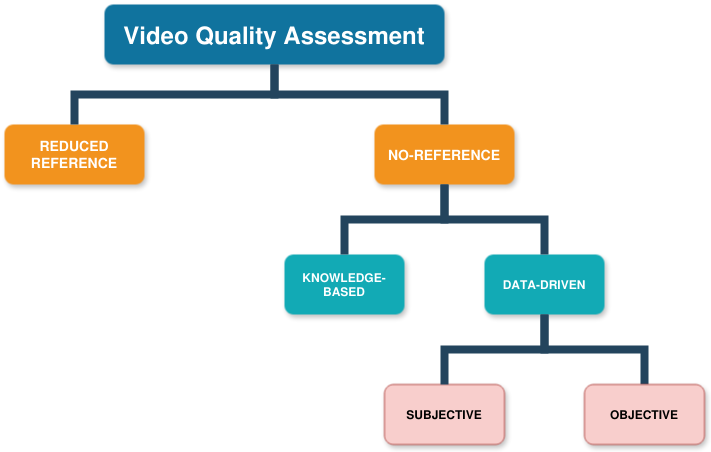
\includegraphics[width=0.86\textwidth]{figures/vqa_diagram.png}
    \caption{Visual Quality Assessment diagram}
    \label{fig:arch}
\end{figure}

\begin{table}[ht]
\centering
\caption{Performance comparison of FastVQA and MDVSFA on different databases. Spearman's Rank Correlation Coefficient (SRCC) and Pearson Linear Correlation Coefficient (PLCC).}
\label{tab:fastvqa_mdvsfa_comparison}
\begin{tabular}{lccc}
\hline
\textbf{Algorithm} & \textbf{Dataset} & \textbf{SRCC} & \textbf{PLCC} \\
\hline
FastVQA & KoNViD-1k    & 0.891 & 0.892 \\
FastVQA & LIVE-VQC     & 0.865 & 0.865 \\
FastVQA & YouTube-UGC  & 0.855 & 0.852 \\
\hline
MDVSFA  & KoNViD-1k    & 0.781 & 0.785 \\
MDVSFA  & LIVE-VQC     & 0.773 & 0.780 \\
MDVSFA  & YouTube-UGC  & 0.749 & 0.746 \\
\hline
\end{tabular}
\end{table}

The Dual-Stage Attention approach introduces a novel architecture that processes video quality assessment in two distinct attention-driven stages \cite{jia2024continuous}. In the first stage, it focuses on spatial features within frames, while the second stage emphasizes temporal relationships across sequential frames, allowing it to capture both spatial distortions and temporal inconsistencies that affect perceived quality. As shown in Table~\ref{tab:dsa_performance}, the Dual-Stage Attention model achieves impressive performance across multiple datasets, particularly when utilizing combined MSE and PLCC loss functions. Meanwhile, DA-QoE (Domain-Adaptive Quality of Experience) employs a weakly supervised learning framework that addresses the domain gap between different datasets, enabling more generalizable quality predictions across diverse video content \cite{li2022weakly}. This is particularly valuable when training data may not fully represent real-world conditions. Table~\ref{tab:da_qoe_performance} further illustrates DA-QoE's strong correlation with human perceptual judgments.

\begin{table}[ht]
\centering
\caption{Performance of Dual-Stage Attention model on different databases. Spearman's Rank Correlation Coefficient (SRCC) and Pearson Linear Correlation Coefficient (PLCC).}
\label{tab:dsa_performance}
\begin{tabular}{lccc}
\hline
\textbf{Dataset} & \textbf{SRCC} & \textbf{PLCC} \\
\hline
Waterloo-IV & 0.795 & 0.801 \\
Waterloo-III & 0.851 & 0.870 \\
LIVE-NFLX-II  & 0.915 & 0.922 \\
\hline
\end{tabular}
\end{table}

\begin{table}[ht]
\centering
\caption{Performance of DA-QoE model on different databases. Spearman's Rank Correlation Coefficient (SRCC) and Pearson Linear Correlation Coefficient (PLCC).}
\label{tab:da_qoe_performance}
\begin{tabular}{lccc}
\hline
\textbf{Dataset} & \textbf{SRCC} & \textbf{PLCC} \\
\hline
LIVE-Mobile-II & 0.7890 & 0.7985 \\
Waterloo SQoE-II & 0.8963 & 0.9156 \\
LIVE Netflix  & 0.8280 & 0.8144 \\
\hline
\end{tabular}
\end{table}

These characteristics make all four algorithms well-suited for the proposed framework, which aims to address real-time quality assessment requirements. The position of these algorithms, alongside other VQA methodologies, is illustrated in the broader context of VQA branches and approaches in Figure~\ref{fig:arch}.

\section{Dissertation Structure} \label{sec:struct}

The structure of this document is organized into five comprehensive chapters. Chapter~\ref{chap:ch2} provides a thorough \textit{Background and Literature Review on State-of-the-Art Video Quality Assessment Algorithms}, exploring key concepts and foundational prior research in the field, offering an in-depth analysis of current methodologies and their applications. Chapter~\ref{chap:ch3} presents the \textit{Preliminary Work and Workplan}, detailing a strategic roadmap for future efforts in this research. Finally, Chapter~\ref{chap:ch4} concludes the document with a summary, highlighting the implications of the work and suggesting directions for further exploration.

 
\chapter{Background and Literature Review} \label{chap:ch2}

\section{Quality of Experience and Methodologies for Video Quality Assessment}  

\subsection{Quality of Experience (QoE): A Holistic Framework}  
Quality of Experience (QoE) has emerged as a multidimensional framework for evaluating multimedia services, 
which encompasses technical, perceptual, and contextual factors that collectively define end-user satisfaction ~\cite{itu2012recommendation}. 
Unlike traditional Quality of Service (QoS) metrics, which focus solely on network performance (e.g., latency, packet loss), 
QoE integrates human-centric elements such as user expectations, emotional engagement, and situational context ~\cite{brunnstrom2013qualinet}. 
Within this framework, video quality remains a critical determinant of QoE, as visual fidelity directly impacts viewer retention and satisfaction, 
particularly in applications such as streaming services, video conferencing, and immersive media ~\cite{wang2004ssim}.

\subsection{Video Quality Assessment Paradigms}  
Video Quality Assessment (VQA) methodologies are broadly categorized into two paradigms, each addressing distinct requirements and constraints.  

\begin{itemize}  
    \item \textbf{Subjective Assessment:} Regarded as the "ground truth" for perceptual quality, subjective evaluation relies on human observers to rate video quality using standardized protocols such as the Absolute Category Rating (ACR) or Double-Stimulus Impairment Scale (DSIS) defined in ITU-R BT.500 \cite{itu2012recommendation}. These methods yield metrics like the Mean Opinion Score (MOS), which quantifies perceived quality on a standardized scale (e.g., 1–5). However, subjective assessments are labor-intensive, costly, and impractical for real-time systems due to their reliance on controlled environments and large participant cohorts.  

    \item \textbf{Objective Assessment:} Objective methods employ computational models to predict quality automatically, enabling scalable and real-time evaluations. These approaches are further classified into:  
    \begin{itemize}  
        \item \textbf{Full-Reference (FR):} Compares distorted content against a pristine reference (e.g., PSNR, SSIM).  
        \item \textbf{Reduced-Reference (RR):} Uses partial reference data (e.g., feature vectors).  
        \item \textbf{No-Reference (NR):} Operates without reference signals, ideal for live-streaming and broadcast monitoring.  
    \end{itemize}  
\end{itemize}  

\subsection{The Case for No-Reference Video Quality Assessment}  
This dissertation focuses on \textbf{No-Reference (NR) VQA}, a critical enabler for real-time quality monitoring in applications where reference content is unavailable or impractical to obtain (e.g., live sports streaming, user-generated content platforms). NR methods infer quality directly from distorted signals using machine learning, deep neural networks, or perceptual models, balancing computational efficiency with prediction accuracy \cite{min2024perceptual}. The absence of reference data, however, introduces challenges such as:  
\begin{itemize}  
    \item \textbf{Content Dependency:} Algorithms must generalize across diverse video genres (e.g., animations, natural scenes).  
    \item \textbf{Distortion Complexity:} Real-world distortions (e.g., compression artifacts, motion blur) often coexist, complicating feature extraction.  
    \item \textbf{HVS Alignment:} Models must mimic human perception to ensure meaningful quality scores \cite{wang2004ssim}.  
\end{itemize}  

\subsection{Foundational Objective Metrics}  
\label{subsec:metrics}  
Objective metrics serve as the backbone for developing and benchmarking NR models. Two widely adopted FR metrics are:  

\subsubsection{Peak Signal-to-Noise Ratio (PSNR)}  
\begin{equation}  
\text{PSNR} = 10 \cdot \log_{10}\left(\frac{\text{MAX}^2}{\text{MSE}}\right)  
\label{eq:psnr}  
\end{equation}  
PSNR quantifies the logarithmic ratio between the maximum pixel value ($\text{MAX}$, typically 255 for 8-bit images) and the Mean Squared Error ($\text{MSE}$) between reference ($x$) and distorted ($y$) frames:  
\[  
\text{MSE} = \frac{1}{N} \sum_{i=1}^{N} (x_i - y_i)^2,  
\]  
where $N$ is the total number of pixels. Despite its simplicity, PSNR correlates poorly with human perception, as it ignores structural distortions and contextual relevance \cite{huynh2012scope}.  

\subsubsection{Structural Similarity Index (SSIM)}  
\begin{equation}  
\text{SSIM}(x, y) = \frac{(2 \mu_x \mu_y + C_1)(2 \sigma_{xy} + C_2)}{(\mu_x^2 + \mu_y^2 + C_1)(\sigma_x^2 + \sigma_y^2 + C_2)}  
\label{eq:ssim}  
\end{equation}  
SSIM, introduced by Wang et al. \cite{wang2004ssim}, addresses PSNR's limitations by modeling three perceptual components:  
\begin{itemize}  
    \item \textbf{Luminance ($\mu_x, \mu_y$):} Mean intensity, reflecting brightness similarity.  
    \item \textbf{Contrast ($\sigma_x, \sigma_y$):} Standard deviation, capturing texture and edge variations.  
    \item \textbf{Structure ($\sigma_{xy}$):} Covariance, assessing spatial correlation between $x$ and $y$.  
\end{itemize}  
The constants $C_1$ and $C_2$ stabilize the computations in regions with low intensity. SSIM ranges from $-1$ (dissimilar) to $1$ (identical), with higher values indicating superior quality. Extensions like 3D-SSIM \cite{zeng2012_3dssim} enhance its utility for video by incorporating temporal dynamics, while multiscale implementations (MS-SSIM) improve robustness to resolution changes \cite{wang2003multiscale}.  

\subsection{Evolution to Data-Driven NR VQA}  
The limitations of hand-made metrics such as PSNR and SSIM have led to the adoption of data-driven NR models. Modern approaches leverage:  
\begin{itemize}  
    \item \textbf{Deep Neural Networks (DNNs):} Architectures such as ResNet \cite{he2016deep} and Vision Transformers (ViTs) \cite{dosovitskiy2020image} extract spatiotemporal features directly from distorted videos.  
    \item \textbf{Hybrid Frameworks:} Combine traditional metrics with machine learning (e.g., MDVSFA \cite{li2023unified} uses ResNet-50 for feature extraction).  
    \item \textbf{End-to-End Optimization:} Models like FastVQA \cite{wu2022fastvqa} prioritize computational efficiency for real-time applications.  
\end{itemize}  
These advances underscore the shift from heuristic models to adaptive, learning-based systems capable of addressing the complexity of in-the-wild video distortions \cite{min2024perceptual}. 

\section{State-of-the-Art Video Quality Assessment Algorithms}\label{sec:se21}

As summarized by a recent survey~\cite{min2024perceptual}, several objective No-Reference Video Quality Assessment (NR VQA) algorithms have demonstrated exceptional performance on commonly used databases. These state-of-the-art algorithms are predominantly based on frameworks built using Deep Neural Networks (DNN), which form the central focus of this study. 

One of these high-performing algorithms, proposed by Wu, Chen, Hou, et al., and referred to as FastVQA~\cite{wu2022fastvqa}, utilizes a unique framework designed for efficient end-to-end video quality assessment. The framework implements fragment sampling to extract critical spatiotemporal features from video sequences, reducing computational complexity while maintaining high-quality predictions. By leveraging an end-to-end training architecture, FastVQA is particularly well-suited for real-time video quality assessment applications, where speed and accuracy are critical. The framework described for this algorithm is highlighted in Figure ~\ref{fig:framework1} and can be described by the two following aspects, which are Grid Mini-patch Sampling (GMS) and the Fragment Attention Network (FANet).

\begin{figure}
    \centering
    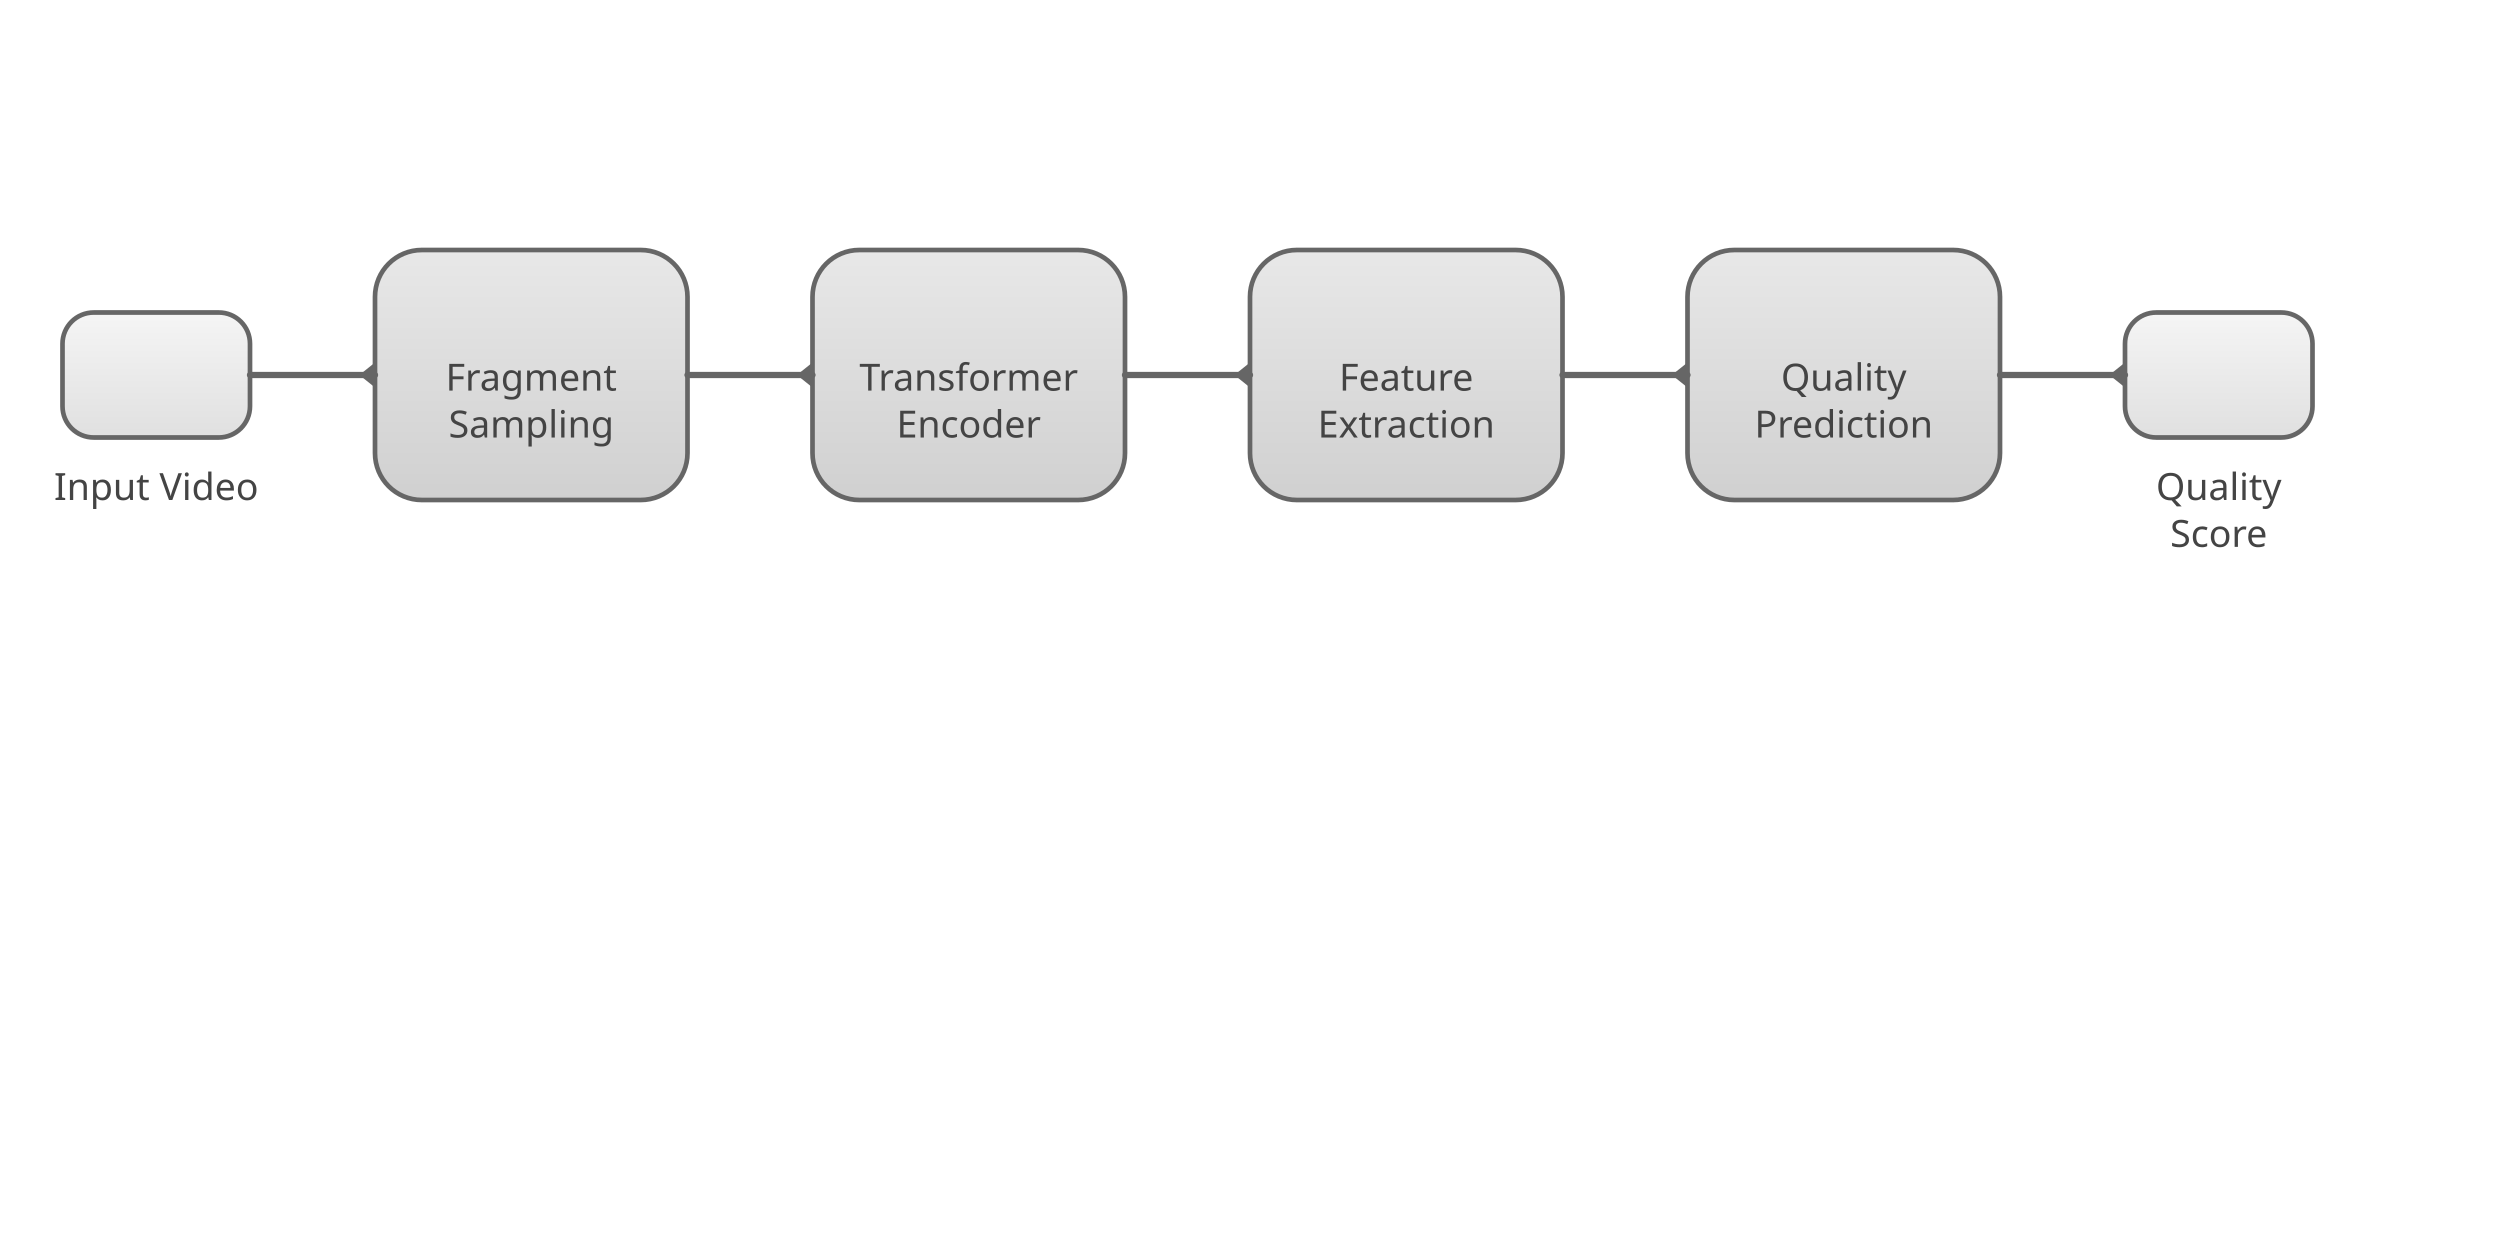
\includegraphics[width=0.9\textwidth]{figures/fast-vqa-framework-3.png}
    \caption{Framework of the algorithm proposed by Wu, Chen, Hou, et al.~\cite{wu2022fastvqa}}
    \label{fig:framework1}
\end{figure}

Grid Mini-patch Sampling (GMS) is a technique designed to capture both global and local video quality features while maintaining efficiency. The process begins by dividing video frames into a uniform grid, preserving global quality. Each frame is divided into smaller grids \(G_f \times G_f\), ensuring that every region of the frame is uniformly assessed, as shown in Equation~\ref{eq:gms_grid}. This grid partition ensures that quality is evaluated in all regions, providing a thorough and balanced analysis.

\begin{equation}
G_f = \frac{\text{Frame Width}}{\text{Grid Size}}, \quad G_f = \frac{\text{Frame Height}}{\text{Grid Size}}
\label{eq:gms_grid}
\end{equation}

To preserve local video quality, raw resolution mini-patches are selected from each grid without resizing, maintaining the original texture of the frame. This helps to retain fine-grained details, such as blurring, noise, and artifacts, which are essential for accurate Video Quality Assessment (VQA). The patches, denoted by $MP_{i,j_t}$, are sampled randomly from each grid, ensuring that the local textural information is captured effectively.

For temporal quality, the sampling process guarantees that patches from different frames are aligned temporally, ensuring consistency across frames. This alignment ensures that the raw temporal variations, which influence the video quality, are retained throughout the entire video sequence. The temporal alignment is enforced by applying the same sampling operation to corresponding regions of each frame, as stated in Equation~\ref{eq:temporal_alignment}.

\begin{equation}
P_t(i, j) = P_{t-1}(i, j) + \Delta_t
\label{eq:temporal_alignment}
\end{equation}

Lastly, the process maintains contextual relations by splicing the sampled mini-patches back into their original positions. This ensures that the global and contextual relationships between patches are preserved, enabling an accurate prediction of overall video quality. The resulting fragments, denoted as $F_{i,j_t}$, are processed further in the subsequent stages of the pipeline.

The Fragment Attention Network (FANet) processes the fragments produced by GMS to predict the video quality. FANet leverages a hierarchical Swin Transformer (Swin-T) backbone, which incorporates four self-attention layers. These layers are designed to efficiently handle both spatial and temporal relationships within the video fragments. FANet introduces two key innovations: Gated Relative Position Biases (GRPB) and Intra-Patch Non-Linear Regression (IP-NLR).

Gated Relative Position Biases (GRPB) are introduced to differentiate between intra-patch and cross-patch attention pairs. In a traditional Swin-T model, a single relative position bias is applied to all attention pairs. However, in the context of fragmented video patches, the distances between patches within the same grid (intra-patch) are much smaller compared to those between patches from different grids (cross-patch). To address this, GRPB employs two distinct bias tables: one for intra-patch pairs (\(T_{\text{real}}\)) and another for cross-patch pairs (\(T_{\text{pseudo}}\)). The gating mechanism, denoted by \(G_{i,j}\), ensures that the appropriate bias is applied depending on whether the attention pair belongs to the same mini-patch or not. This approach allows FANet to capture both local and global quality relationships accurately.

Intra-Patch Non-Linear Regression (IP-NLR) is designed to handle the discontinuities between mini-patches, which may exhibit diverse qualities. Direct pooling across different mini-patches could confuse the quality representations. To avoid this, IP-NLR processes the features through non-linear layers (denoted as RNL) before applying pooling. This ensures that each patch's quality representation is independently processed before pooling, preventing the blending of features from patches with varying qualities.

The final output of FANet is a video quality score ($s_{pred}$) that reflects the overall perceptual quality of the video. By combining the fine-grained sampling approach of GMS with the advanced attention mechanisms of FANet, the FAST-VQA framework provides an effective method for no-reference video quality assessment.

Another high-performing algorithm, the MDVSFA framework, was proposed by Li, Jiang, and Jiang in~\cite{li2023unified}. Unlike FastVQA, this framework incorporates a pre-trained ResNet-50 model as its backbone for content-aware and distortion-sensitive feature extraction. The MDVSFA framework is illustrated in Figure~\ref{fig:framework2}, highlighting its three-stage design: Relative Quality Assessor, Nonlinear Mapping, and Dataset-Specific Perceptual Scale Alignment.

\begin{figure}
\centering
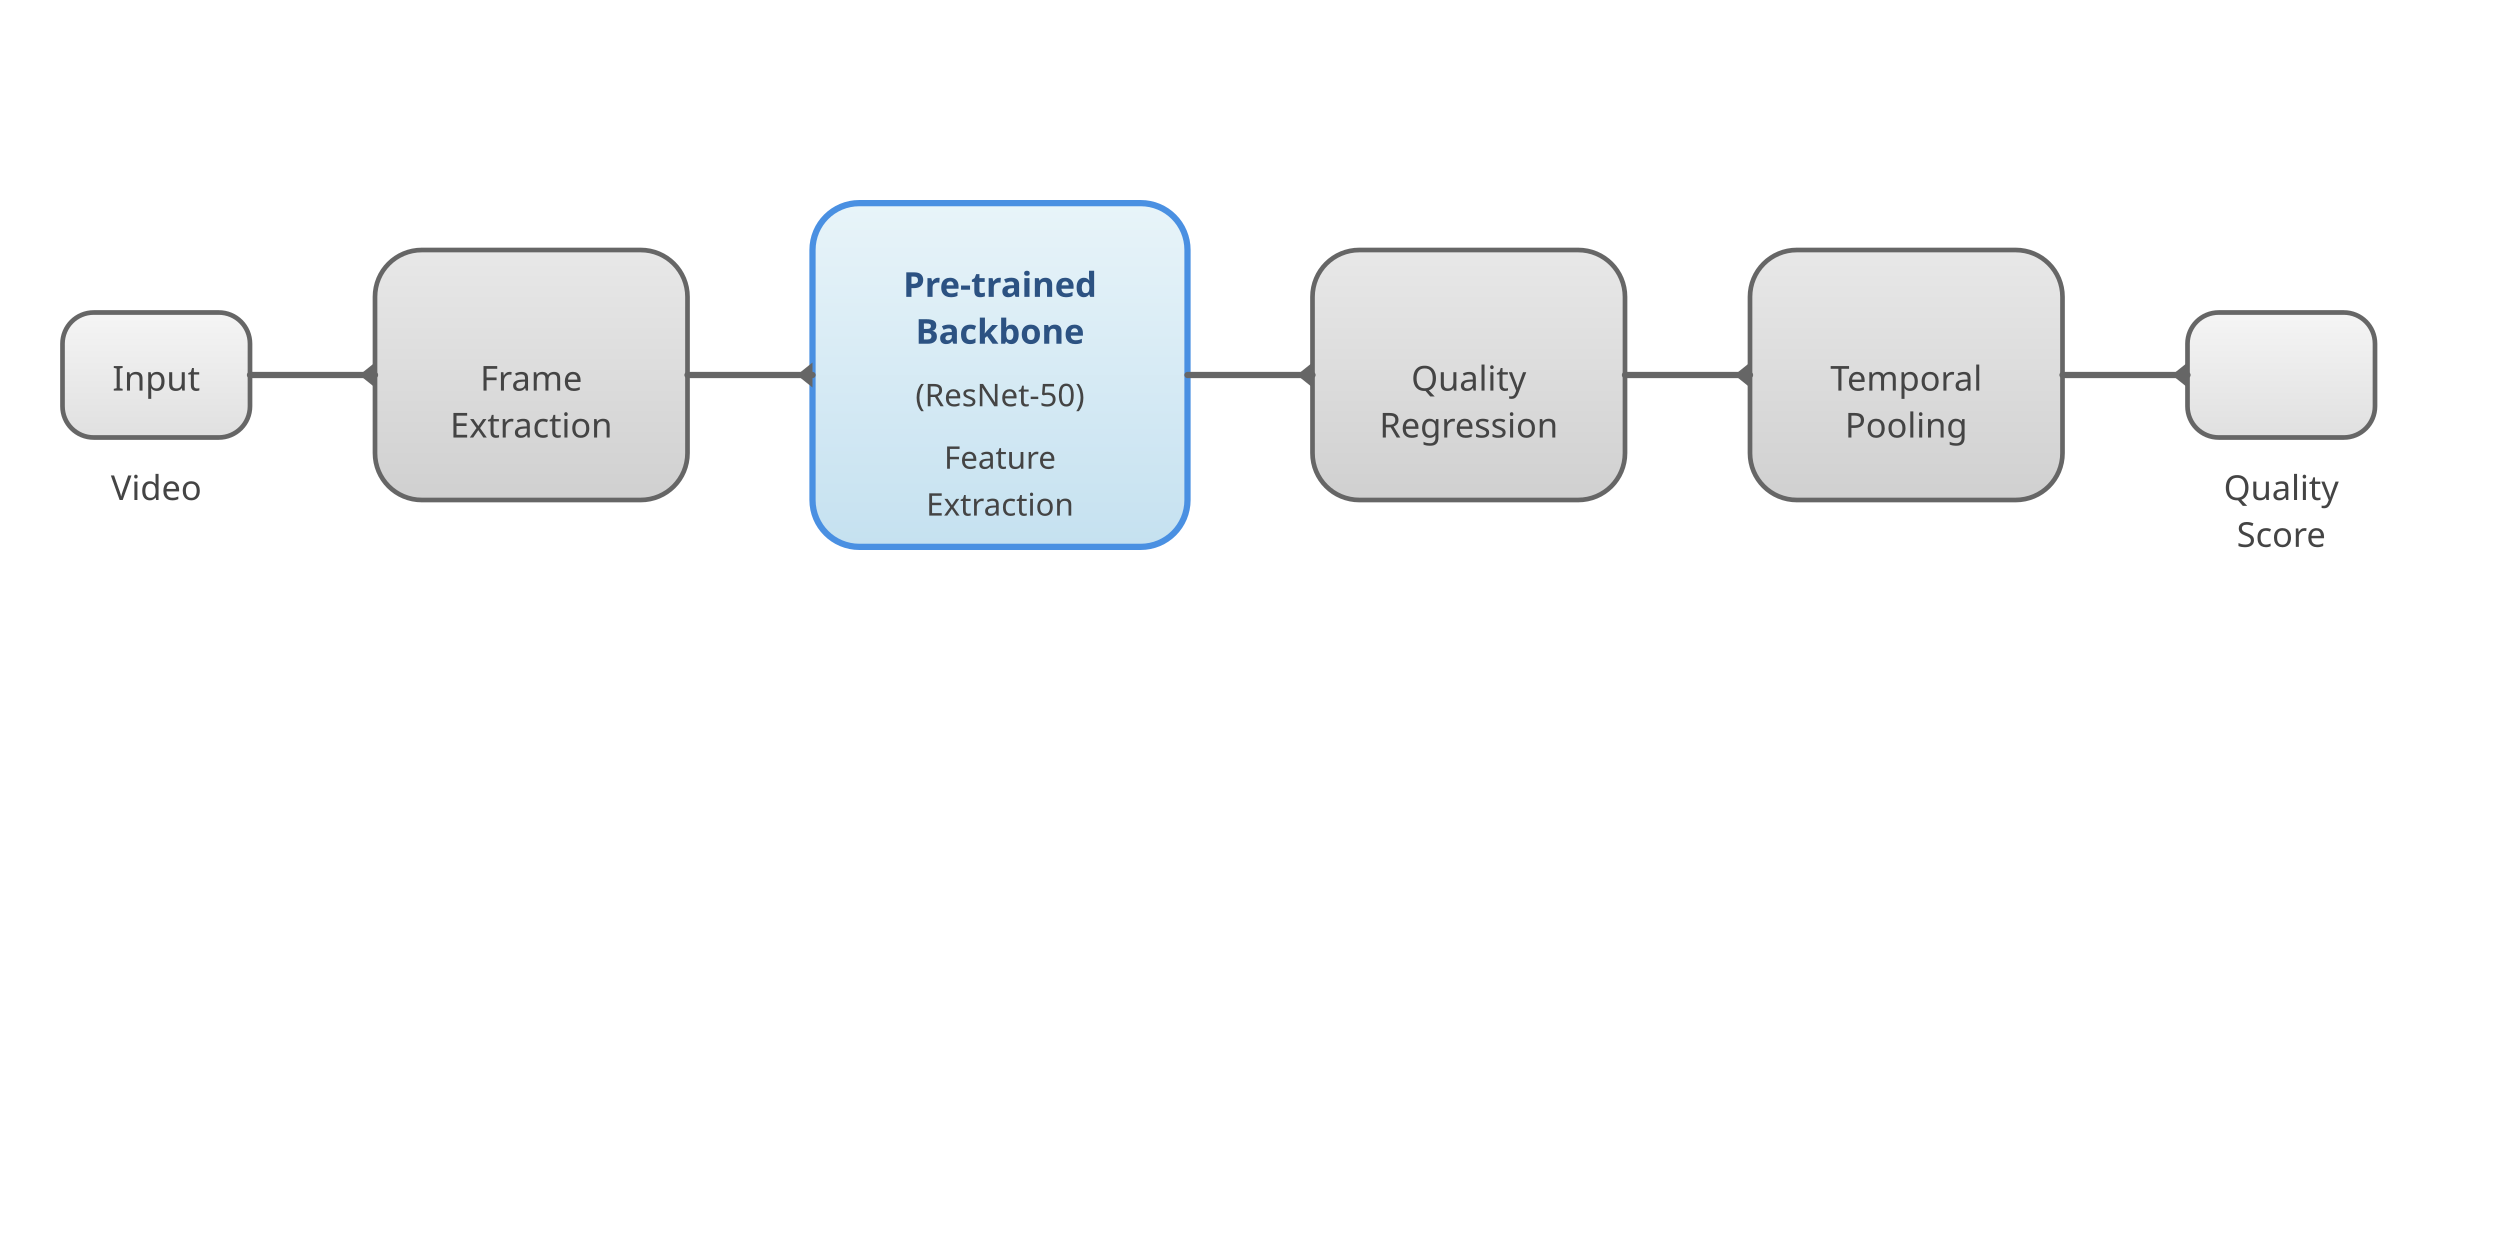
\includegraphics[width=0.9\textwidth]{figures/unified-vqa-framework-3.png}
\caption{Framework of the MDVSFA algorithm proposed by Li, Jiang, and Jiang~\cite{li2023unified}}
\label{fig:framework2}
\end{figure}

The first stage, Relative Quality Assessor, extracts content-aware features from video frames using ResNet-50, followed by temporal integration using a GRU network to model the temporal-memory effect. This stage is supervised by a monotonicity-induced loss, ensuring that the predicted quality ranks are consistent with subjective rankings.

In the second stage, Nonlinear Mapping a four-parameter logistic function is implemented to account for the nonlinearity in human visual perception. This mapping transforms the relative quality scores into perceptual quality scores while maintaining linear correlations with subjective quality, guided by a linearity-induced loss.

Finally, the third stage, Dataset-Specific Perceptual Scale Alignment, addresses inconsistencies in subjective quality score ranges across datasets. A dataset-specific alignment layer maps perceptual quality scores to subjective quality scores specific to each dataset. This alignment is supervised by an error-induced loss, allowing mixed datasets to be utilized effectively during training.

Overall, the MDVSFA framework offers a unified approach to VQA by addressing content dependency, temporal-memory effects, and dataset-specific discrepancies, demonstrating superior performance on multiple in-the-wild datasets~\cite{li2023unified}.

Another high-performing algorithm is the dual-stage attention model proposed by Jia et al.~\cite{jia2024continuous}, specifically designed for continuous and overall Quality of Experience (QoE) evaluation in streaming video. Unlike previous approaches, this model addresses the unique challenges of streaming content, where temporal variations in quality significantly impact user experience. The framework, illustrated in Figure~\ref{fig:framework3}, consists of two primary components: rich feature exploration and dual-stage attention mechanisms.

\begin{figure}
\centering
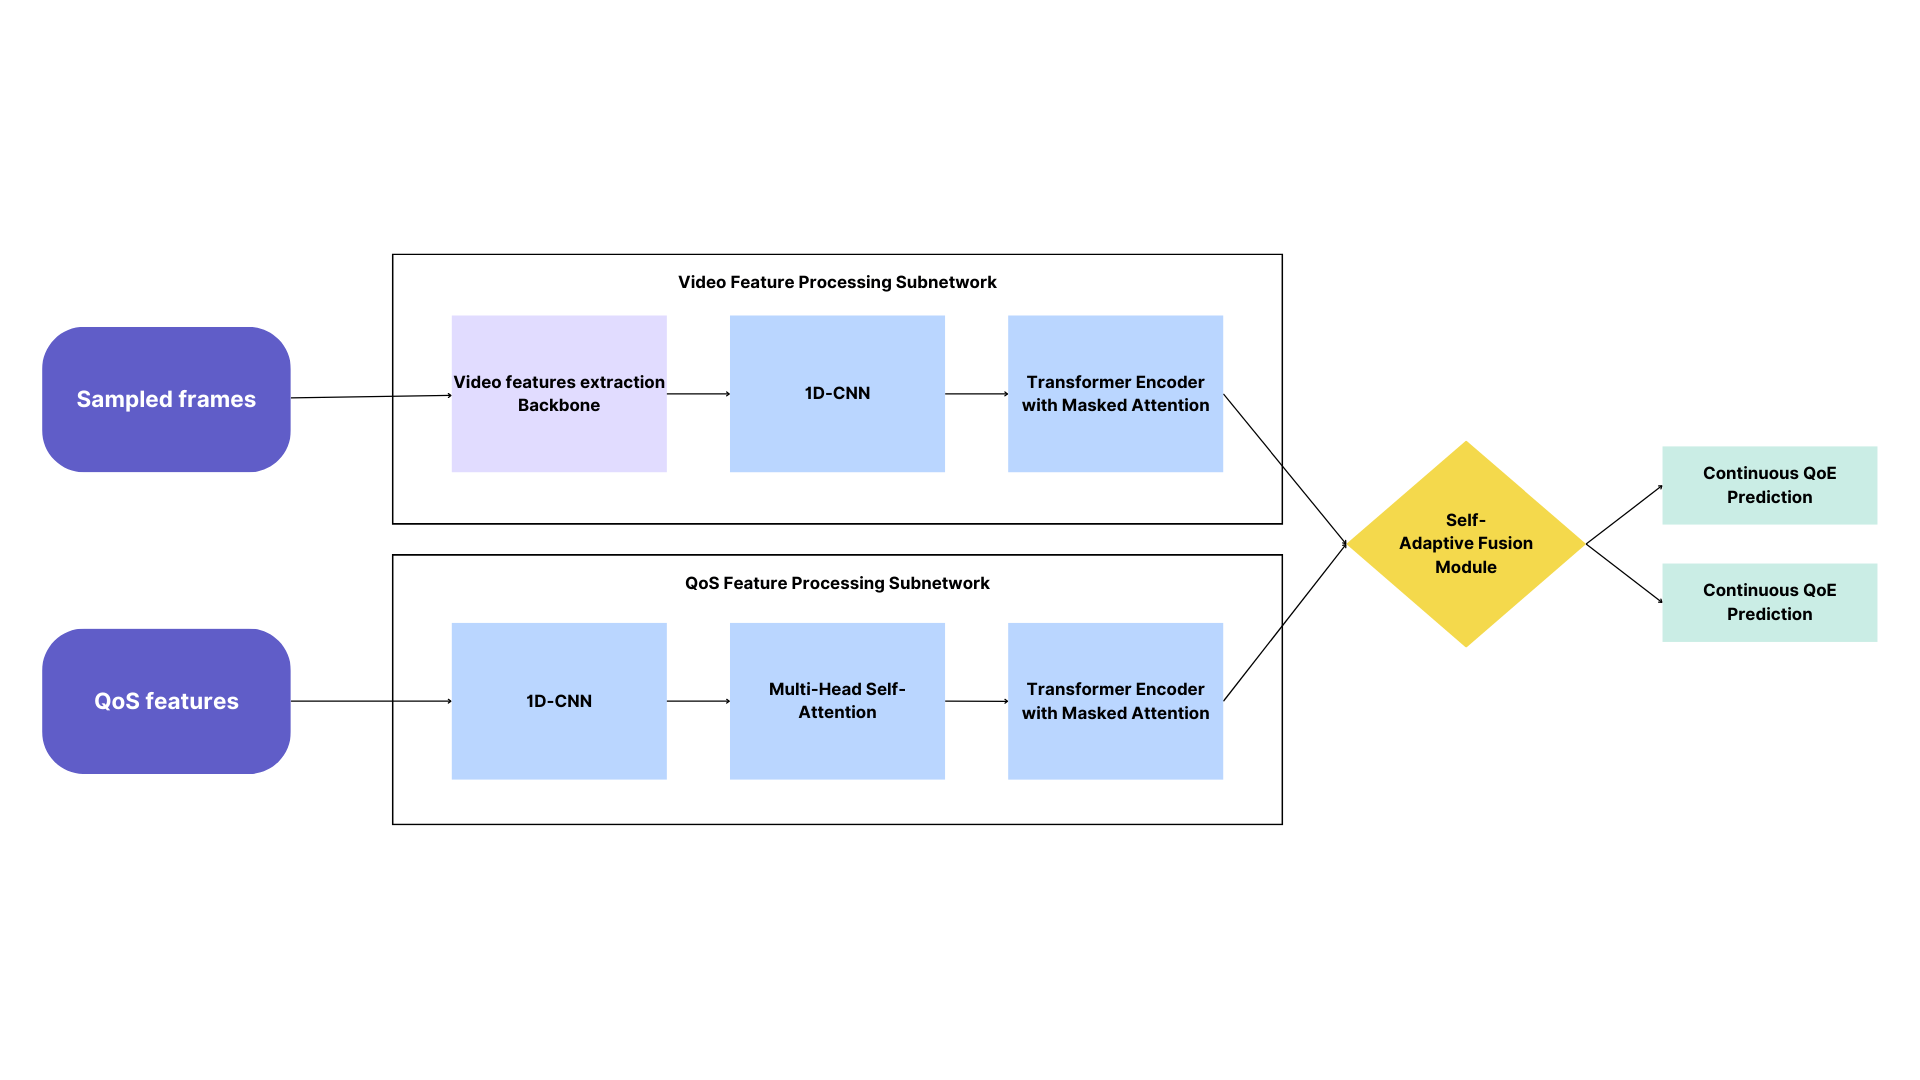
\includegraphics[width=0.9\textwidth]{figures/dual-attention-framework.png}
\caption{Framework of the dual-stage attention model for streaming QoE proposed by Jia et al.~\cite{jia2024continuous}}
\label{fig:framework3}
\end{figure}

To bridge the gap between perceptual video quality and user Quality of Experience (QoE) in streaming scenarios, Jia et al.~\cite{jia2024continuous} propose a unified architecture for both overall and continuous QoE prediction. Their model integrates high-level semantic content features and low-level Quality of Service (QoS) indicators using a dual-stage attention mechanism. 

The architecture comprises two parallel subnetworks: a \textit{video content feature stream} and a \textit{QoS feature stream}. Spatial features are extracted using the final four stages of a pretrained ResNet-50 backbone, while motion features are obtained via the Fast path of a SlowFast network pretrained on Kinetics-400. These are temporally aggregated via global average and standard deviation pooling and concatenated into a 7936-dimensional vector.

The QoS stream encodes time-varying features such as stalling duration, bitrate value, temporal recency of playback disruptions, and bitrate switching dynamics. These features are processed with a grouped 1D-CNN, followed by a \textit{cross-feature attention} (CFA) module based on multi-head self-attention, which captures dependencies among QoS groups and models perceptual non-linearities.

Both feature streams are processed through short-time regression (STR) modules to model short-term quality dynamics, and long-time regression (LTR) modules consisting of Transformer encoder blocks with masked attention to capture long-range temporal dependencies. A \textit{self-adaptive fusion module} then computes a weighted combination of both streams, where the weights are learned as a function of content–QoS interactions. This fusion produces either overall QoE (via temporal pooling and regression) or continuous QoE (frame-level outputs with timestep-wise adaptive fusion).

This model achieves superior performance across multiple public streaming QoE datasets, and its architecture directly reflects key perceptual principles such as content-dependent quality sensitivity and hierarchical processing of temporal and spatial features, making it a strong candidate for real-time QoE inference pipelines.

\section{Algorithms' Performance and Implementation Justification}  
\label{sec:performance_conclusions}

The rapid evolution of adaptive video streaming technologies has necessitated robust methodologies for continuous Quality of Experience (QoE) monitoring. In this work we focus on three state‐of‐the‐art no‐reference VQA/QoE frameworks already introduced in Section 2.2: MDVSFA \cite{li2023unified}, FastVQA \cite{wu2022fastvqa}, and the dual‐stage attention model \cite{jia2024continuous}. Each model embodies distinct design trade‐offs in feature extraction, temporal modeling, and deployment efficiency.

\subsection{Methodological Overview}  
MDVSFA \cite{li2023unified} employs a pretrained ResNet-50 backbone to extract multi‐scale spatial features from each frame, integrates temporal context via a GRU, and aligns model outputs to subjective scores through a three‐stage pipeline: relative quality ranking (monotonicity loss), nonlinear perceptual mapping (linearity loss), and dataset‐specific scale alignment (error‐induced loss). This mixed‐dataset training yields strong cross‐dataset generalization.  

FastVQA \cite{wu2022fastvqa} introduces Grid Mini‐patch Sampling (GMS) to fragment each frame into raw‐resolution patches, preserving local textures and global structure. A Fragment Attention Network (FANet) built on a hierarchical Swin Transformer processes these fragments, using Gated Relative Position Biases (GRPB) to distinguish intra‐ vs.\ cross‐patch attention, and Intra‐Patch Non‐Linear Regression (IP-NLR) to avoid feature discontinuity before pooling. FastVQA achieves real‐time inference with minimal accuracy loss.  

Dual-Stage Attention \cite{jia2024continuous} unifies continuous and overall QoE prediction by fusing high‐level semantic features (ResNet-50 + SlowFast) with low‐level QoS indicators (stall duration, bitrate changes, recency). Short‐time and long‐time temporal regression modules capture local and global temporal dynamics, while a Cross‐Feature Attention (CFA) module models perceptual non‐linearities among QoS groups. A self‐adaptive fusion layer then learns content–QoS weighting for final QoE scores.

\subsection{Comparative Analysis and Selection Rationale}  
MDVSFA’s mixed‐dataset alignment affords strong cross‐dataset performance but relies on frame‐level ranking supervision, which can overlook fine‐grained temporal artifacts. FastVQA’s fragment sampling is codec-agnostic and preserves spatial details, yet its short fragment windows may underrepresent long‐term quality drift. The dual-stage attention model explicitly integrates both spatial–temporal features and QoS logs, yielding robust performance across streaming scenarios.  

FastVQA addresses only fragment‐level temporal consistency via aligned patch sampling, whereas MDVSFA relies on GRU memory, which can accumulate error over long sequences. Dual-stage attention combines dedicated STR (short-time) and LTR (long-time) modules with masked self‐attention, capturing both transient stalls and prolonged bitrate shifts with human‐aligned weighting.  

On modern GPU hardware, FastVQA processes 1080p video at over 30 FPS due to its lightweight fragment pipeline. MDVSFA’s ResNet-50 + GRU chain runs at 15 FPS for full‐resolution frames. The dual-stage attention model incurs higher per‐frame cost (20 ms/frame) but remains within real‐time budgets when optimized and crucially supports continuous QoE outputs.

Given the need for a unified, codec-agnostic, perceptually accurate and temporally comprehensive QoE predictor—yet still deployable under real‐time constraints—we select the dual-stage attention architecture as the centerpiece of this dissertation. Its explicit modeling of both low-level QoS and high-level semantic distortions, combined with dual temporal regression and adaptive fusion, aligns most closely with professional streaming requirements and the goals of this study.  

\section{Neural Networks for Quality-of-Experience Prediction}  
\label{sec:nn_qoe}  

The advent of deep learning has revolutionized Video Quality Assessment (VQA) by enabling data-driven approaches that directly model the complex relationship between video distortions and human perceptual judgments. This section examines neural network architectures specifically engineered for Quality of Experience (QoE) prediction, focusing on their capacity to emulate human visual perception while meeting the computational demands of real-time applications. Unlike generic computer vision models, these architectures incorporate specialized mechanisms to address the unique challenges of perceptual quality assessment, particularly in no-reference scenarios where reference content is unavailable.

\subsection{Architectural Paradigms for Perceptual Quality Prediction}  
Contemporary QoE-driven VQA systems predominantly employ two neural network paradigms, each offering distinct advantages for modeling different aspects of visual quality perception:

\begin{itemize}  
    \item \textbf{Convolutional Neural Networks (CNNs):} These architectures excel at extracting hierarchical spatial features through their localized receptive fields, making them particularly effective at identifying common video artifacts such as blocking, blurring, and banding \cite{he2016deep}. Their inductive biases for translation invariance and local connectivity align well with the Human Visual System's (HVS) early processing stages.
    
    \item \textbf{Vision Transformers (ViTs):} By leveraging self-attention mechanisms, ViTs capture long-range spatiotemporal dependencies that are crucial for modeling global quality perception \cite{dosovitskiy2020image}. Their ability to dynamically weight different regions of the video frame mimics the HVS's attention mechanisms, making them particularly suitable for assessing complex distortions that span multiple spatial and temporal scales.
\end{itemize}  

State-of-the-art implementations typically employ a hybrid approach, where networks are pre-trained on large-scale multimedia datasets (e.g., ImageNet, Kinetics) and subsequently fine-tuned for VQA-specific tasks \cite{li2023unified}. This transfer learning paradigm enables robust feature representation while mitigating the data scarcity challenges inherent to perceptual quality assessment.

\subsection{Case Study: Hierarchical Feature Extraction with ResNet-50}  
The framework proposed by Li \textit{et al.}~\cite{li2023unified} serves as an exemplary implementation of CNN-based QoE prediction, demonstrating how traditional computer vision architectures can be adapted for perceptual quality assessment. The system employs a two-stage processing pipeline that addresses both low-level distortion detection and high-level quality estimation:

\begin{enumerate}  
    \item \textbf{Multi-Scale Spatiotemporal Feature Extraction:}  
    \begin{itemize}  
        \item The ResNet-50 backbone processes individual video frames through its convolutional layers, generating a hierarchy of feature maps that capture distortions at varying spatial scales (from pixel-level artifacts to frame-wide impairments).
        \item Temporal dynamics are modeled through a combination of 3D convolutions and recurrent units (GRUs), which aggregate features across successive frames to account for motion-related distortions and temporal masking effects \cite{lee2021video}.
    \end{itemize}  
    
    \item \textbf{Feature Normalization and Quality Regression:}  
    \begin{itemize}  
        \item Domain-specific normalization techniques (e.g., instance normalization with learned parameters) are applied to mitigate dataset biases arising from varying resolutions, bitrates, and content types.
        \item Spatial average pooling generates compact, content-agnostic feature descriptors that feed into a quality regression head, which predicts MOS scores through fully connected layers.
    \end{itemize}  
\end{enumerate}  

This architecture demonstrates how traditional CNN designs can be effectively repurposed for perceptual quality assessment by incorporating temporal modeling and domain adaptation components.

\subsection{Optimizing for Perceptual Alignment}  
Achieving accurate quality prediction requires careful alignment between computational models and human perceptual mechanisms. Modern QoE-driven VQA systems address this through two principal strategies: advanced loss function design and biologically-inspired attention mechanisms.

The design of perceptually-weighted loss functions extends beyond conventional mean squared error (MSE) optimization. Recent work by \cite{min2024perceptual} demonstrates that incorporating temporal weighting factors accounts for the recency effect in human quality judgments, where viewers tend to disproportionately weight the quality of recent video segments. Additionally, content-adaptive weighting schemes emphasize distortion visibility in perceptually critical regions, such as areas with high spatial frequency content or salient objects, while reducing emphasis on less visually important regions. These approaches mirror findings from psychovisual studies showing that human quality perception is non-uniform across both spatial and temporal dimensions.

Attention mechanisms play a particularly crucial role in bridging the gap between artificial quality assessment and human perception. As demonstrated by \cite{wu2022fastvqa}, spatial and channel attention modules dynamically modulate feature importance based on distortion visibility, effectively mimicking the Human Visual System's (HVS) selective attention processes. Neuropsychological research has shown that the HVS employs similar mechanisms to prioritize processing of visually salient regions while suppressing less relevant information \cite{itti1998model}. In VQA systems, this manifests as learned attention patterns that emphasize:
\begin{itemize}
    \item Texture-rich regions where compression artifacts are most visible
    \item Motion boundaries affected by temporal compression
    \item High-contrast edges susceptible to ringing artifacts
\end{itemize}
This biological plausibility contributes to the models' ability to predict subjective quality judgments with high accuracy, as evidenced by their strong correlation with Mean Opinion Scores (MOS) across diverse content types and distortion profiles. 

\subsection{Implementation Challenges and Practical Considerations}  
Despite their demonstrated effectiveness, neural network-based QoE predictors face several persistent challenges that influence architectural choices and deployment strategies:

\begin{itemize}  
    \item \textbf{Data Scarcity and Annotation Costs:} The labor-intensive nature of subjective quality assessment severely limits dataset sizes, with most public benchmarks containing fewer than 1,000 annotated sequences \cite{hosu2020konvid}. This scarcity is compounded by the domain gap between different datasets, as noted by \cite{li2023unified}. Recent approaches address these limitations through several strategies: robust cross-dataset training frameworks that learn domain-invariant features, semi-supervised techniques leveraging unlabeled data, and synthetic data generation methods that preserve perceptual quality relationships. The MDVSFA architecture \cite{li2023unified} demonstrates particular effectiveness in cross-dataset scenarios through its unified quality assessment paradigm.
    
    \item \textbf{Computational Complexity:} Vision Transformers (ViTs) achieve state-of-the-art performance but require significant computational resources due to their quadratic complexity with respect to input size \cite{liu2021swin}. Their deployment typically necessitates powerful GPU hardware, though recent advances in model compression techniques have improved their practicality. Quantization methods, for instance, can reduce model size and computation requirements by using lower-precision arithmetic without significant quality prediction degradation. Efficient attention variants like shifted window approaches and hybrid CNN-Transformer architectures offer additional pathways for balancing accuracy and computational demands.
    
    \item \textbf{Interpretability and Explainability:} The black-box nature of deep quality predictors complicates their adoption in production environments. While techniques like Grad-CAM \cite{selvaraju2017grad} provide post-hoc explanations by visualizing spatial contributions to quality predictions, more intrinsic interpretability remains an open research challenge. This is particularly crucial for applications requiring quality-based decision making, where stakeholders need to understand the rationale behind quality scores.
\end{itemize}  

\section{Rust and Machine Learning Inference in Media Pipelines}

Although most machine learning (ML) inference pipelines are traditionally implemented in high-level languages such as Python or in low-level C/C++ stacks, the Rust programming language has emerged as a promising alternative for system-level deployment of real-time media and AI applications. Rust's emphasis on safety, concurrency, and performance makes it a suitable candidate for time-sensitive, memory-safe environments like media streaming infrastructures.

One important development in this direction is the growing use of \textbf{GStreamer}, an open-source multimedia pipeline framework that has become a standard in many Linux-based distributions and platforms. As noted in Ham et al.~\cite{ham2019nnstreamer}, ``GStreamer~\cite{gstreamer1999} is the standard multimedia pipeline framework for Tizen and many Linux distributions. GStreamer provides APIs and utilities to construct stream pipelines for multimedia applications of various platforms including Linux, Android, Windows, iOS, and macOS. GStreamer is highly modular; every filter and path control is implemented as a plugin attached in run-time. GStreamer has been applied to various systems where multimedia performance matters. BBC uses GStreamer for their broadcasting system.''

In particular, the NNStreamer project~\cite{ham2019nnstreamer} extends GStreamer to integrate neural network inference directly into the media pipeline by treating trained ML models as stream filters. This approach streamlines the execution of deep learning models on-device and serves as an important precedent for real-time AI-augmented media processing.

While GStreamer has traditionally relied on C and C++, recent developments have demonstrated the feasibility of integrating Rust into these pipelines. The modularity and runtime plugin architecture of GStreamer make it particularly conducive to Rust-based components, providing the opportunity for safer and more reliable media applications.

Despite Rust’s increasing popularity, gaps remain in the academic and industrial literature regarding its use in real-time ML inference for media pipelines. As noted by Beltrán-Escobar et al.~\cite{beltran2024review}, Rust's adoption in embedded systems and computer vision has accelerated in recent years, especially within the TinyML community. However, they emphasize that “no low- or large-scale commercial and industrial applications using Rust language for real-time image processing and control systems have been reported.” This underscores the need for empirical studies and practical implementations that explore Rust’s capabilities in this domain.

Further, a recent systematic survey by Sharma et al.~\cite{sharma2023rust} highlights both the promise and the challenges of using Rust in embedded environments. Their findings suggest that while Rust addresses many traditional safety pitfalls in C-based embedded systems, its ecosystem maturity and integration with advanced ML toolchains are still evolving.

In light of this context, this dissertation offers a novel contribution by implementing a state-of-the-art neural network model for no-reference video quality assessment (NR-VQA) in a Rust-based media pipeline. It serves as an exploratory trial to bridge the gap between research and deployment, extending the practical knowledge base for using Rust in AI-augmented multimedia systems, with relevance for both embedded and cloud-scale scenarios.

\section{Synthesis and Architectural Innovations}

Several recent deep VQA/QoE models have pushed the state-of-the-art while highlighting different design trade‑offs. \textbf{FAST-VQA} (Wu \textit{et al.}, 2022) uses a grid-based ``fragment'' sampling of raw-resolution patches and a dedicated fragment-attention transformer (FANet) to capture local and global quality cues. This end-to-end model achieves $\approx$10\% accuracy gains over prior VQA methods while dramatically reducing compute for high-resolution videos~\cite{wu2022fastvqa}. \textbf{MDTVSFA} (Li \textit{et al.}, 2021) addresses the cross-dataset problem by training a single model on mixed VQA datasets. It explicitly models human perception (content dependency and temporal memory) and includes stages of relative quality assessment, nonlinear mapping, and dataset-specific perceptual scale alignment~\cite{li2023unified}. This unified approach demonstrated superior cross-dataset performance compared to specialized models~\cite{li2023unified}. In contrast, some streaming-QoE models (e.g. \textit{DA-QoE}) combine hand-crafted QoS and visual features with recurrent networks to predict QoE scores, but often rely on explicit network or compression statistics and lack deep perceptual modeling~\cite{li2022weakly}.

Most of these advances focus on off-line VQA accuracy on standard datasets, and few explicitly target the constraints of real-time content distribution. For example, Bampis and Bovik observe that conventional VQA metrics fail to predict human QoE when streaming impairments like rebuffering and bitrate changes occur~\cite{BAMPIS2018218}. In practice, live streaming requires low-latency, high-reliability assessments that account for temporal attention and episodic events (e.g. stalls), which many models do not handle. FAST-VQA and MDTVSFA are powerful but primarily designed for static evaluation rather than continuous playback scenarios. Likewise, models like DA-QoE or GCNN-QoE use statistical features and GRUs, which may not fully capture perceptual nuance or may introduce latency in inference.

The \textbf{dual-stage attention} approach of Jia \textit{et al.} (2024) bridges these gaps. Their DSA-QoE network explicitly models temporal attention and cross-feature attention to predict \textit{continuous} QoE alongside overall scores~\cite{jia2024continuous}. In experiments on multiple streaming QoE datasets, this model significantly outperforms prior methods, underscoring the value of human-like attention mechanisms in QoE prediction. Because it is a no-reference, codec-agnostic model focused on perceptual quality, it is well-suited to real-world streaming content.

Over the past decade, deep learning–based no‐reference video quality assessment (NR‐VQA) and Quality of Experience (QoE) models have achieved remarkable progress by leveraging increasingly sophisticated feature extraction and temporal modeling techniques. The FastVQA framework introduced by Wu \textit{et al.}~\cite{wu2022fastvqa} exemplifies an efficiency‐oriented design: by fragmenting each frame into raw‐resolution patches via Grid Mini‐patch Sampling (GMS) and processing these through a hierarchical Swin Transformer–based Fragment Attention Network (FANet), FastVQA attains a nearly 10\% improvement in Spearman’s rank correlation over prior methods while sustaining real‐time throughput for high‐resolution video input. However, despite its compelling balance of spatial fidelity and computational efficiency, FastVQA’s short‐window fragment sampling is not explicitly attuned to the episodic temporal distortions—such as rebuffering stalls and bitrate variations—that critically shape viewer experience in live streaming applications.

In contrast, the MDVSFA model proposed by Li \textit{et al.}~\cite{li2023unified} addresses the challenge of cross‐dataset generalization through a unified, mixed‐dataset training strategy. MDVSFA employs a pretrained ResNet‐50 backbone to extract multi‐scale spatial feature maps and integrates temporal context via a Gated Recurrent Unit (GRU). Its three‐stage supervision—comprising relative quality ranking (monotonicity loss), nonlinear perceptual mapping (linearity loss), and dataset‐specific scale alignment (error‐induced loss)—enables the model to produce MOS predictions that remain well‐calibrated across diverse video domains. Nevertheless, the reliance on GRU‐based temporal aggregation can lead to drift when modeling long‐duration sequences, and the absence of explicit mechanisms for modeling low‐level playback metrics limits its sensitivity to critical streaming impairments.

The dual‐stage attention architecture of Jia \textit{et al.}~\cite{jia2024continuous} synthesizes the strengths of both high‐level content modeling and low‐level QoS feature integration within a unified framework tailored for continuous and overall QoE prediction. In this scheme, semantic features are extracted from the final four stages of a ResNet‐50 backbone and from the fast pathway of a SlowFast network pretrained on Kinetics‐400, while QoS features—including stalling indicators, bitrate representations, temporal recency, and bitrate switch dynamics—are processed through grouped 1D‐CNNs to preserve feature‐wise granularity. Short‐time and long‐time temporal regression modules, respectively implemented via masked 1D convolutions and Transformer‐based masked self‐attention, capture both immediate and protracted temporal dependencies. A cross‐feature attention (CFA) module further models the perceptual non‐linearities among QoS feature groups, and a self‐adaptive fusion mechanism learns content–QoS weighting to produce final QoE scores. Empirical evaluations demonstrate that this model attains Spearman’s rank correlations up to 0.89 on live streaming datasets, outperforming both FastVQA and MDVSFA in capturing real‐world streaming anomalies.

In summary, while FastVQA~\cite{wu2022fastvqa} and MDVSFA~\cite{li2023unified} have advanced the frontiers of efficient spatial–temporal feature extraction and cross‐dataset robustness, respectively, they lack dedicated mechanisms for jointly modeling network‐induced impairments and perceptual feature fusion over varying temporal scales. Conversely, the dual‐stage attention model~\cite{jia2024continuous} provides a comprehensive solution by integrating semantic and QoS streams through hierarchical attention and adaptive fusion, thereby reconciling the demands of low‐latency inference, perceptual fidelity, and codec‐agnostic deployment. These characteristics render it the most suitable foundation for real‐time QoE monitoring in professional audiovisual distribution pipelines.

Jia et al.’s dual-stage attention architecture emerges as the most viable solution, harmonizing accuracy, efficiency, and adaptability. Its ability to localize distortion-prone regions via attention maps not only enhances interpretability but also aligns with human visual saliency, making it uniquely suited for deployment in dynamic, multi-codec streaming platforms. The selection of this model is further vindicated by its modular design, which facilitates seamless integration into existing media pipelines without requiring architectural overhauls—a critical consideration for industry adoption.

To complement this architectural innovation, the implementation of this model within a Rust-based media pipeline represents a novel contribution to the systems-level deployment of real-time QoE solutions. Rust's strong guarantees of memory and concurrency safety, zero-cost abstractions, and absence of garbage collection provide the necessary foundations for high-performance streaming applications~\cite{fulton2022benefits}. Its integration within modular frameworks such as GStreamer has been increasingly explored, and its feasibility for embedded machine learning inference has been demonstrated by projects like MicroFlow~\cite{carnelos2025microflow}. Despite its growing academic presence, recent reviews~\cite{beltran2024review,sharma2023rust} point out a lack of reported large-scale deployments in real-time media processing systems. By embedding DSA-QoE within a Rust-powered inference pipeline, this dissertation not only tests the architectural strengths of dual-stage attention but also addresses a gap in the literature regarding the operational viability of Rust for AI-augmented multimedia applications.
\chapter{From Design to Deployment: Transitioning to Full Implementation} \label{chap:ch3}

\section{Model Architecture Development}

This dissertation has progressed through the complete implementation, training, and deployment lifecycle of a real-time video Quality of Experience (QoE) prediction system. The core objective was to validate whether a state-of-the-art model, such as the Dual-Stage Attention network (DSA-QoE)~\cite{jia2024continuous}, could be operationalized in a production-grade media pipeline entirely powered by the Rust programming language.

The previously selected DSA-QoE architecture was first implemented and trained using the PyTorch framework in Python, exploiting its rich ecosystem for deep learning development and GPU-accelerated training. After achieving stable learning dynamics and acceptable generalization performance on a benchmark dataset, the trained model was serialized using TorchScript and deployed via the \texttt{tch-rs} crate into a Rust-native application layer designed for real-time media inference.

The transition from experimental setup to operational deployment involved overcoming significant engineering challenges, including stream buffer management, multi-threaded tensor pre-processing under real-time constraints, and integration with GStreamer based video pipelines. These were addressed using Rust's advanced safety guarantees—such as memory and concurrency correctness through the ownership model—and by leveraging its zero-cost abstractions for performance-critical sections.

This chapter presents not only the architecture and development work, but also a complete exposition of the system's final configuration, including real-time implementation details. The successful end-to-end execution of the inference pipeline in Rust, maintaining throughput close to source frame rate and latency within acceptable bounds, demonstrates the language's applicability in high-performance AI-driven media systems. Furthermore, this implementation contributes empirical validation to ongoing academic discussions about the use of Rust in safety-critical AI workloads~\cite{fulton2022benefits, johansson2023transitioning, carnelos2025microflow}.

\section{Dataset Implementation and Preprocessing}

To train and validate the Dual-Stage Attention (DSA-QoE) model, this work employs the LIVE-NFLX-II dataset~\cite{live_nflx_conf}, a curated benchmark for perceptual quality assessment under realistic video streaming conditions. The dataset provides frame-accurate annotations for both retrospective Mean Opinion Scores (MOS) and continuous perceptual quality, as well as low-level Quality of Service (QoS) metrics such as bitrate switching and playback interruptions. These properties make it ideal for modeling perceptual Quality of Experience (QoE) in dynamic and bandwidth-constrained environments.

\subsection{Custom PyTorch Dataset Class}

The implementation of data loading and processing is encapsulated in a custom PyTorch \texttt{Dataset} class. Upon initialization, all dataset annotations are parsed from pickled metadata files (\texttt{*.pkl}), which contain temporal MOS vectors, video durations, distortion types, and playback metadata. From these, video durations are measured and global normalization parameters are computed for both QoS features and labels.

Each distorted video is loaded using \texttt{EncodedVideo} from \texttt{PyTorchVideo}~\cite{fan2021pytorchvideodeeplearninglibrary}, allowing efficient frame decoding and time-based clip segmentation. Videos are processed in fixed-length segments of $T = 10$ seconds, with start and end times incremented accordingly.

\subsection{Dual Transformation Pipeline}

The preprocessing consists of a dual-pathway transformation architecture implemented in the \texttt{Transform} class. Each video segment undergoes two independent transformations: a SlowFast oriented Transform, which applies time-aligned sampling and resolution changes to produce dual-pathway inputs and a ResNet oriented Transform, that generates temporally sampled frame sequences for static spatial processing.

These transformations are implemented using \texttt{ApplyTransformToKey} from \texttt{PyTorchVideo} ~\cite{fan2021pytorchvideodeeplearninglibrary}, with the video tensor accessed via the \texttt{"video"} key. 

Each transformation applies the following operations:

\paragraph{SlowFast Transform.}
\begin{enumerate}
    \item \texttt{UniformTemporalSubsample($T$)} to extract a fixed number of evenly spaced frames.
    \item \texttt{Lambda(lambda x: x/255.0)} to scale raw pixel intensities to the $[0, 1]$ range.
    \item \texttt{NormalizeVideo(mean, std)} to normalize each RGB channel.
    \item \texttt{Resize()} to reduce spatial resolution for efficient training.
    \item \texttt{PackPathway()} to split frames into a slow and fast pathway for the SlowFast model. The \texttt{PackPathway} module selects every $\frac{1}{\alpha}$-th frame for the slow pathway using linear index sampling, where $\alpha$ was set to 4. The remaining high-rate frames form the fast pathway. The result is a list of tensors: \texttt{[slow\_pathway, fast\_pathway]}.
\end{enumerate}

\paragraph{ResNet Transform}
\begin{enumerate}
    \item \texttt{UniformTemporalSubsample($T$)} to select representative frames.
    \item Pixel normalization to $[0,1]$ and per-channel standardization.
    \item No resizing is applied in this transform, preserving original resolution.
\end{enumerate}

These transformations yield two parallel streams:
\begin{align*}
x_{\text{slowfast}} &= [\text{slow\_pathway}, \text{fast\_pathway}] \\
x_{\text{resnet}}   &= \text{stack of temporally sampled frames}
\end{align*}

\subsection{QoS Feature Processing and Label Normalization}

In parallel with video processing, a set of four QoS time series is extracted for each clip:
\begin{itemize}
    \item \texttt{playback\_indicator}
    \item \texttt{temporal\_recency}
    \item \texttt{representation\_quality}
    \item \texttt{bitrate\_switch}
\end{itemize}

These features are min-max normalized using statistics computed from the full dataset:
\[
\hat{q}_{i,j} = \frac{q_{i,j} - \min(q_j)}{\max(q_j) - \min(q_j)}
\]

Similarly, the labels—both the scalar retrospective MOS and the frame-wise continuous MOS—are normalized across the dataset using per-type bounds. This target normalization mitigates differences in scale across output variables, ensuring that no single regression objective dominates the optimization process. As discussed in Chapter 7 of Goodfellow et al. ~\cite{goodfellow2016deep}, normalization of targets in regression tasks helps maintain stable gradient magnitudes, accelerates convergence, and contributes to more balanced multi-objective learning.

\subsection{Output Structure and Caching with \texttt{PickleDataset}}

The final data returned from \texttt{VideoDataset} includes:
\begin{verbatim}
{
  'video_content': (slowfast_tensor, resnet_tensor),
  'qos': qos_features,
  'overall_QoE': overall_mos,
  'continuous_QoE': temporal_mos
}
\end{verbatim}

To reduce data loading time, the \texttt{PickleDataset} subclass adds caching functionality. Each sample is preprocessed once, serialized with \texttt{torch.save()}, and saved in \texttt{assets\_cached/}. Future runs retrieve these preprocessed tensors via \texttt{torch.load()}, greatly improving training throughput in subsequent epochs.

\section{Model Overview and Modular Design}

The Dual-Stage Attention for Quality of Experience (DSA-QoE) prediction model integrates multiple sub-modules into a cohesive architecture designed to predict continuous and retrospective QoE scores from both high-level semantic video content and low-level Quality of Service (QoS) indicators. Figure ~\ref{fig:framework3} illustrates the structural layout of the proposed model, comprising two parallel processing branches---a video content feature subnetwork and a QoS feature subnetwork---which are ultimately merged by a feature fusion module.

The \textbf{video content feature subnetwork} is responsible for capturing spatial and temporal information from the visual stream. It includes the \textit{Rich Feature Extraction Backbone}, composed of a dual-pathway network---a ResNet-50 for spatial semantics as introduced by He et al. ~\cite{he2016deep} and SlowFast for motion dynamics as introduced by Feichtenhofer et al. ~\cite{feichtenhofer2019slowfast}---, followed by the \textit{Short-Time Regression Module} and \textit{Long-Time Regression Module} to model short-term and long-term temporal dependencies, respectively. These modules independently process perceptual features derived from the visual stream without incorporating external QoS data.

Conversely, the \textbf{QoS feature subnetwork} operates on temporal sequences of streaming metrics such as stalling duration, bitrate variation, and playback recency. This branch includes not only analogous \textit{Short-Time} and \textit{Long-Time Regression Modules}, but also an intermediate \textbf{Cross-Feature Attention Module}, inspired by the self-attention paradigm~\cite{vaswani2017attention}, to model complex interdependencies among QoS features. This structural asymmetry reflects the need for perceptual non-linear modeling in the QoS domain, where interpretability and weighting of features vary temporally and contextually ~\cite{jia2024continuous}.

After the respective regressions in each subnetwork, the model employs a \textbf{Feature Fusion Module}, which computes a self-adaptive combination of the content and QoS representations. This module enables synergistic integration of perceptual and systemic quality cues and facilitates both frame-level (continuous) and global (retrospective) QoE prediction. The fused representation is finally passed through \textbf{Fully Connected Networks} to output the final quality predictions.

To summarize, the model architecture comprises the following main components:
\begin{itemize}
\item \textbf{Rich Feature Extraction Backbone}: Extracts spatial and motion features from raw video.
\item \textbf{Short-Time Regression Module}: Captures local temporal variations in perceived quality.
\item \textbf{Cross-Feature Attention Module}: Applies only to the QoS subnetwork to capture inter-feature dependencies.
\item \textbf{Long-Time Regression Module}: Models prolonged temporal dependencies via Transformer encoders.
\item \textbf{Feature Fusion Module}: Merges content and QoS feature representations.
\item \textbf{Fully Connected Networks}: Regress the fused representation to final QoE outputs and reduces the feature vector dimensionality after the rich feature extraction.
\end{itemize}

This layered, modular construction not only mirrors the human perceptual process in handling audiovisual stimuli and delivery impairments, but also allows for fine-grained inspection and modification of each stage. The following subsections provide in-depth technical details and implementation specifics for each module listed above.

\subsection{Rich Feature Extraction Backbone}

This section details the design and implementation of the feature extraction backbone used in the Dual-Stage Attention QoE prediction model~\cite{jia2024continuous}. The backbone is structured as a dual-pathway encoder: one pathway for extracting spatial-semantic content from individual video frames using a ResNet-50~\cite{he2016deep}, and the other for encoding motion dynamics from temporally sampled video clips using the SlowFast network~\cite{feichtenhofer2019slowfast}, pretrained on the Kinetics-400 dataset~\cite{kay2017kineticshumanactionvideo}. 

The dual-pathway design enables the model to simultaneously learn frame-level perceptual attributes and motion-sensitive cues, both of which are essential for no-reference QoE estimation in real-time streaming contexts. All source code associated with this implementation, including both the Python-based model development and the Rust-based inference deployment, is publicly available at \url{https://github.com/cthadeufaria/dual-stage-attention}.

The perceptual backbone comprises two pretrained convolutional models whose outputs are concatenated and passed into the temporal attention and fusion modules. During training, both networks are frozen to minimize overfitting and reduce GPU memory usage.

\subsubsection{Motion Feature Pathway}

The motion feature pathway is implemented using the SlowFast architecture, accessed via the \texttt{pytorchvideo} ~\cite{fan2021pytorchvideodeeplearninglibrary} library. SlowFast is designed to process video at two temporal resolutions:
\begin{itemize}
    \item The \textbf{slow pathway} receives sparsely sampled frames to capture high-level semantic motion patterns.
    \item The \textbf{fast pathway} receives densely sampled frames with fewer channels to detect fine-grained motion.
\end{itemize}

In this implementation, we follow the sampling setup used in DSA-QoE: temporal stride $\tau=6$, channel ratio $\beta=8$, and speed ratio $\alpha=4$. These parameters control the spatial-temporal granularity of motion representation and ensure alignment with the perceptual distortions commonly found in streaming media.

To extract motion features, the model registers forward hooks on each \texttt{ResNetBlock} module in the SlowFast architecture. A forward hook in PyTorch is a callback that intercepts the output of a layer during the forward pass. This allows intermediate activations to be stored without altering the model's computation graph. Formally, the hook is defined via:
\begin{quote}
\texttt{layer.register\_forward\_hook(hook\_fn)}
\end{quote}
where \texttt{hook\_fn} is a function of signature \texttt{(module, input, output)}. In this model, the hook stores the output tensors in a class-wide dictionary keyed by layer index.

After inference, the activation from the fourth residual stage (\texttt{Fi[4]}) is selected and passed through a global 3D average pooling:
\[
\texttt{motion\_features} = \texttt{AdaptiveAvgPool3d}((1,1,1))(\texttt{Fi[4]})
\]
This operation reduces the spatial-temporal tensor to a compact latent vector that is flattened and returned for downstream concatenation. The entire operation is wrapped in \texttt{torch.inference\_mode()} to ensure memory safety and prevent autograd overhead.

\subsubsection{Semantic Feature Pathway}

The semantic feature extractor uses a ResNet-50 model pretrained on the ImageNet dataset~\cite{5206848}, accessed via \texttt{torchvision}. To reduce training time and avoid overfitting, the model is frozen and set to evaluation mode. The final four residual stages of the ResNet (layers 2 to 5) are manually indexed and accessed for feature extraction. Forward hooks are registered to these layers using:
\begin{quote}
\texttt{layer.register\_forward\_hook(hook\_fn)}
\end{quote}
where the hook function saves the output activation in a dictionary using the number of input channels as a unique key. This method follows best practices outlined in \cite{nanbhasblog,torchhooksdoc} for forward hook registration and layer-specific activation access.

Given the activation maps $F_i = \{f_{i,1}, f_{i,2}, f_{i,3}, f_{i,4}\}$ from the four ResNet stages, the semantic vector is constructed by applying:
\begin{itemize}
    \item \textbf{Global Average Pooling (GAP)} across spatial dimensions to capture average filter response.
    \item \textbf{Pooled Standard Deviation (PStd)} to encode activation dispersion.
\end{itemize}

Formally:
\[
\alpha_i = \texttt{cat}\left( \left\{\texttt{GAP}(f_{i,j})\right\}_{j=1}^{4} \right),
\quad
\beta_i = \texttt{cat}\left( \left\{\texttt{std}(f_{i,j})\right\}_{j=1}^{4} \right),
\quad
F'_i = \texttt{cat}(\alpha_i, \beta_i)
\]

This results in a robust representation of both intensity and variance of the high-level features, which together enhance the model's sensitivity to structural and perceptual distortions in each frame. The semantic feature pathway operates on spatially aligned individual frames sampled from the video input and is evaluated in tandem with the motion pathway during inference.

\subsection{Short-Time Regression Module}

The Short-Time Regression (STR) module is implemented to capture local temporal dependencies within the QoE feature sequences. This design is motivated by Temporal Convolutional Networks (TCNs) introduced by Bai et al.~\cite{bai2018empirical}, which have been shown to outperform recurrent architectures like LSTMs in sequence modeling tasks due to their parallelism and stable gradient behavior.

This module consists of two parallel 1D-CNN variants—\texttt{Simple1DCNN} and \texttt{Group1DCNN}—each designed to process different feature modalities while preserving temporal length.

In the \texttt{Simple1DCNN} branch, used for video content features, three sequential convolutional blocks with kernel width 5 are applied to the tensor of shape $(T, 180)$. Each block consists of left-zero-padding of 4, a \texttt{Conv1d}(180 → 180), and \texttt{ReLU}. The repeated convolutional layers enable a receptive field that spans short time intervals, providing fine-grained temporal context without collapsing temporal resolution.

The \texttt{Group1DCNN} branch handles QoS features grouped by their semantic type. It uses grouped convolutions to transform a $(T, 4)$ tensor into a $(T, 180)$ representation in two stages: first expanding each QoS group independently (channels 4 → 180), then refining channel-wise features (channels 180 → 180). Grouped convolutions facilitate parallel learning of feature-specific temporal filters, aligning with perceptual theories that distinct QoS signals may affect QoE independently before integration.

Both branches avoid pooling to maintain the same temporal length at the output, enabling direct alignment with the frame- or segment-level QoE supervision. The resulting outputs, reshaped back to $(T, 180)$, are suitable for fusion with long-range temporal dynamics modeled downstream.

This architecture echoes the fundamental TCN design pattern—causal 1D convolutions, dilations or large kernels, and skip connections—that enable rich local contextual modeling while supporting parallel, non-recursive training~\cite{bai2018empirical}. By combining STR and LTR modules, the overall system captures both fine- and broad-scale temporal structures relevant to perceptual quality assessment.

\subsection{Cross-Feature Attention Module}

The Cross-Feature Attention (CFA) module, a method described by Vaswani et al.~\cite{vaswani2017attention}, is employed to model high-order interactions across semantically distinct Quality of Service (QoS) feature groups in a temporally aligned manner. While previous layers encode intra-feature temporal dynamics (e.g., how bitrate varies across time), the CFA module explicitly attends across different QoS groups, enabling the model to infer complex joint effects on perceptual Quality of Experience (QoE). This is crucial for capturing compound distortions that arise in streaming applications, such as simultaneous bitrate drops and stalling events.

The module draws directly from the scaled dot-product attention mechanism proposed by Vaswani et al.~\cite{vaswani2017attention}, where input sequences are projected into queries ($Q$), keys ($K$), and values ($V$), and the attention output is computed as:
\[
\text{Attention}(Q, K, V) = \text{softmax}\left(\frac{QK^T}{\sqrt{d_k}}\right)V
\]
This formulation allows the model to dynamically weight features based on their contextual relevance, thereby enabling global reasoning over the input.

In the CFA module, the input is a matrix $x \in \mathbb {R}^{T \times F}$, where $T$ is the number of temporal segments and $F = 180$ is the flattened dimension of encoded QoS features. The features are grouped into $G=4$ non-overlapping blocks of size $d = F/G = 45$, consistent with the grouping strategy adopted during feature encoding. The tensor is reshaped to $\mathbb{R}^{G \times T \times d}$ and permuted to match the expected input format of PyTorch's \texttt{nn.MultiheadAttention}, i.e., $(\text{seq\_len}, \text{batch}, \text{embed\_dim})$.

Using 3 attention heads, the CFA computes multi-head self-attention across grouped features at each timestep. The heads independently project the input to subspaces of dimension $d_h = d / h = 15$ and apply scaled dot-product attention. The outputs of the attention heads are then concatenated and projected back to the original group dimension, following the standard Transformer procedure~\cite{vaswani2017attention}. This allows each group to attend to other groups over time, yielding a globally informed representation of inter-group dependencies.

The attended tensor is then permuted and flattened back to $\mathbb {R}^{T \times F}$ to be passed to subsequent layers. This operation maintains the temporal structure of the QoS sequence while enriching it with attention-based feature fusion, effectively reweighting the contributions of each group based on contextual cues.

The rationale for integrating such an attention mechanism is supported by the findings of Vaswani et al., who demonstrate that attention not only improves modeling capacity but also reduces the need for strong inductive biases such as recurrence or convolution. In our context, replacing hand-crafted fusion heuristics with a trainable attention mechanism provides greater flexibility and empirical robustness in modeling perceptual impairments.

By applying attention to grouped QoS features, the CFA module leverages the inductive strength of the Transformer architecture to capture how complex combinations of impairments affect perceptual quality. This is consistent with broader observations in the literature that attention mechanisms excel in scenarios requiring dynamic, content-dependent reasoning~\cite{vaswani2017attention}.

\subsection{Long-Time Regression Module}

The Long-Time Regression (LTR) module is a Transformer-based architecture designed to model extended temporal dependencies across perceptual and network features in streaming video sequences. This module is critical for capturing long-range temporal coherence in Quality of Experience (QoE) estimation, particularly when degradations such as bitrate oscillations or stalling have temporally diffuse perceptual impacts.

The module is based on the Transformer Encoder architecture introduced by Vaswani et al.~\cite{vaswani2017attention}, which replaces recurrence with multi-head self-attention and feedforward layers. This architecture has demonstrated superior performance in capturing global dependencies across sequences and is especially well suited to tasks involving temporally structured inputs. In contrast to RNN-based models, Transformer encoders allow for parallel sequence processing and content-based interactions, enhancing both representational power and training efficiency.

The LTR module receives as input a sequence of feature vectors $x \in \mathbb{R}^{T \times D}$, where $T$ denotes the number of time steps (e.g., segment-aligned video windows), and $D = 180$ is the dimensionality of the combined feature representation. To encode temporal order information, the model introduces a learnable positional encoding matrix $P \in \mathbb{R}^{T \times D}$, which is added to the input:
\[
F = x + P
\]

The core of the module is a stack of $L$ Transformer Encoder layers, each consisting of a multi-head self-attention mechanism followed by a feedforward network, residual connections, and layer normalization. Each encoder layer adheres to the following structure:
\[
\text{EncoderLayer}(x) = \text{LayerNorm}(x + \text{SelfAttention}(x)) + \text{FeedForward}(x)
\]
with $H = 4$ attention heads and feedforward dimensionality $4D = 720$, using ReLU as the activation function.

To ensure that predictions at time $t$ do not attend to future information $t' > t$, a causal mask is applied via PyTorch's \texttt{generate\_square\_subsequent\_mask()} function. This constructs a triangular mask matrix $M \in \mathbb{R}^{T \times T}$ such that:
\[
M_{ij} =
\begin{cases}
0, & \text{if } j \leq i \\
-\infty, & \text{if } j > i
\end{cases}
\]
This constraint is essential for autoregressive learning and simulates the causal information flow observed in real-time streaming systems.

The output from the stacked encoder is then projected back to the feature space via a fully connected layer:
\[
O = \text{SELU}(\text{FC}(C)) + C
\]
where $C$ is the Transformer encoder output, and SELU is used as the activation function to preserve self-normalizing behavior and facilitate gradient stability.

Overall, the LTR module integrates long-term perceptual dynamics by propagating content-aware representations through the Transformer encoder. By leveraging positional encoding and masked attention, it maintains both sequential order and causal consistency. As originally shown by Vaswani et al.~\cite{vaswani2017attention}, this architectural design offers a powerful alternative to recurrent approaches, enabling the model to capture the long-horizon structure inherent to human perceptual response in streaming contexts.

\subsection{Feature Fusion Module}

The core of the model's predictive capacity lies in its ability to dynamically integrate heterogeneous data streams—specifically, video content features and Quality of Service (QoS) metrics. To this end, a dedicated Feature Fusion Module (FFM) is designed to leverage both global and local information by applying adaptive weighting mechanisms inspired by dual-stage attention frameworks, as proposed by Jia et al.~\cite{jia2024continuous}.

Formally, let $O_{vc} \in \mathbb{R}^{T \times d}$ denote the temporally-aligned sequence of high-level video content embeddings, and $O_{QoS} \in \mathbb{R}^{T \times d}$ the corresponding QoS feature sequence, both output by the long-time temporal regression modules. These representations encode semantic, motion, and playback characteristics at the chunk level.

We define temporally pooled representations:
\begin{equation}
    X_{vc} = \frac{1}{T} \sum_{t=1}^{T} O_{vc}^{(t)}, \quad 
    X_{QoS} = \frac{1}{T} \sum_{t=1}^{T} O_{QoS}^{(t)},
\end{equation}
which capture the global statistical behavior of each modality.

To compute a self-adaptive fusion weight $\alpha \in (0, 1)$ governing the contribution of each modality to the overall Quality of Experience (QoE) prediction, we concatenate the global descriptors and pass them through a learned fully-connected network $\mathrm{FC}_2$:
\begin{equation}
    \alpha = \mathrm{FC}_2 \left( \mathrm{concat}(X_{vc}, X_{QoS}) \right).
\end{equation}

The fused overall representation is then constructed as a convex combination:
\begin{equation}
    \hat{X}_{ova} = \mathrm{concat} \left( \alpha \cdot X_{vc}, (1 - \alpha) \cdot X_{QoS} \right),
\end{equation}
which is subsequently passed to another fully connected layer $\mathrm{FC}_3$ to predict the overall QoE:
\begin{equation}
    \hat{y}_{ova} = \mathrm{FC}_3(\hat{X}_{ova}).
\end{equation}

For continuous QoE estimation, a similar mechanism is applied on a per-timestep basis. Let the concatenated dynamic features be
\begin{equation}
    Z_t = \mathrm{concat}(O_{vc}^{(t)}, O_{QoS}^{(t)}), \quad t = 1, \dots, T.
\end{equation}
A timestep-dependent fusion weight $\alpha_t$ is computed using another fully connected layer $\mathrm{FC}_4$:
\begin{equation}
    \alpha_t = \mathrm{FC}_4(Z_t),
\end{equation}
leading to timestep-specific fused representations:
\begin{equation}
    \hat{Z}_t = \mathrm{concat} \left( \alpha_t \cdot O_{vc}^{(t)}, (1 - \alpha_t) \cdot O_{QoS}^{(t)} \right),
\end{equation}
which are individually mapped to predicted continuous QoE scores using $\mathrm{FC}_5$:
\begin{equation}
    \hat{y}_t = \mathrm{FC}_5(\hat{Z}_t).
\end{equation}

This fusion strategy serves multiple purposes: it enables context-dependent feature recalibration, alleviates overfitting risks associated with static fusion methods, and mimics the perceptual prioritization seen in human viewers when evaluating content under varying transmission conditions ~\cite{jia2024continuous}. Moreover, the two-stage design reflects both coarse-grained and fine-grained attention to temporal and feature-wise dependencies, contributing to enhanced prediction robustness in both overall and continuous QoE evaluation tasks.

\subsection{Fully Connected Networks}

The architecture integrates five fully connected networks—\texttt{FC1} to \texttt{FC5}—to progressively transform, weight, and regress features throughout the dual-stage attention model. These layers are implemented in PyTorch as subclasses of \texttt{nn.Module}, using best practices from the official PyTorch guidelines ~\cite{pytorch_tutorials}.

\subsubsection*{\texttt{FC1}: Dimensionality Reduction Layer}

The first network, \texttt{FC1}, reduces the high-dimensional concatenated feature vector obtained after rich feature extraction. The input dimensionality of $7936$ results from combining semantic features (from ResNet-50 and SlowFast) and motion features as per the design in ~\cite{jia2024continuous}. To avoid overfitting and reduce computation, \texttt{FC1} maps this to a 180-dimensional latent space:
\begin{equation}
    \hat{f}_t = \texttt{FC1}(f_t), \quad \hat{f}_t \in \mathbb{R}^{180}, \quad f_t \in \mathbb{R}^{7936}.
\end{equation}
In code, this is implemented as a single-layer perceptron:
\begin{verbatim}
self.layer1 = nn.Linear(7936, 180)
\end{verbatim}
No activation function is applied, consistent with its role as a bottleneck projection.

\subsubsection*{\texttt{FC2}: Overall Fusion Weight Estimation}

The second network, \texttt{FC2}, computes a scalar fusion coefficient $\alpha \in (0,1)$ from the concatenated global average pooled features of the video content and QoS sub-networks. It uses a two-layer feedforward network with a \texttt{ReLU} activation followed by a final \texttt{Sigmoid} to bound the output:
\begin{align}
    \alpha &= \sigma\left( W_2 \cdot \texttt{ReLU}(W_1 \cdot x + b_1) + b_2 \right), \\
    x &= \texttt{concat}(X_{vc}, X_{QoS}) \in \mathbb{R}^{360}.
\end{align}
Implemented as:
\begin{verbatim}
self.layer1 = nn.Linear(360, 180)
self.relu = nn.ReLU()
self.layer2 = nn.Linear(180, 1)
self.sigmoid = nn.Sigmoid()
\end{verbatim}
This module enables a content-aware blending of modalities, as discussed in~\cite{jia2024continuous}.

\subsubsection*{\texttt{FC3}: Overall QoE Prediction Layer}

Once the scalar weight $\alpha$ is used to combine pooled feature vectors, the fused vector of 360 dimensions is passed to \texttt{FC3}, which predicts the overall Quality of Experience score:
\begin{equation}
    \hat{y}_{ova} = \texttt{FC3}(\alpha X_{vc} \oplus (1 - \alpha) X_{QoS}).
\end{equation}
\texttt{FC3} comprises two fully connected layers with a non-linear \texttt{GELU} activation ~\cite{hendrycks2016gaussian} in between:
\begin{verbatim}
self.layer1 = nn.Linear(360, 180)
self.gelu = nn.GELU()
self.layer2 = nn.Linear(180, 1)
\end{verbatim}

\subsubsection*{\texttt{FC4}: Per-Timestep Fusion Weight Estimation}

Analogous to \texttt{FC2}, the \texttt{FC4} network estimates fusion weights $\alpha_t$ per timestep, enabling frame-level adaptivity. It takes as input the concatenated representations at timestep $t$ and outputs a scalar $\alpha_t \in (0,1)$:
\begin{equation}
    \alpha_t = \sigma\left( W_2 \cdot \texttt{ReLU}(W_1 \cdot z_t + b_1) + b_2 \right), \quad z_t = O_{vc}^{(t)} \oplus O_{QoS}^{(t)}.
\end{equation}
The implementation mirrors \texttt{FC2}:
\begin{verbatim}
self.layer1 = nn.Linear(360, 180)
self.relu = nn.ReLU()
self.layer2 = nn.Linear(180, 1)
self.sigmoid = nn.Sigmoid()
\end{verbatim}
This mechanism allows the model to express dynamic content-awareness at each timestep ~\cite{jia2024continuous}.

\subsubsection*{\texttt{FC5}: Continuous QoE Prediction Layer}

Finally, \texttt{FC5} maps the dynamically fused features at each timestep to scalar continuous QoE scores:
\begin{equation}
    \hat{y}_t = \texttt{FC5} \left( \alpha_t O_{vc}^{(t)} \oplus (1 - \alpha_t) O_{QoS}^{(t)} \right).
\end{equation}
As with \texttt{FC3}, it employs a \texttt{GELU} activation:
\begin{verbatim}
self.layer1 = nn.Linear(360, 180)
self.gelu = nn.GELU()
self.layer2 = nn.Linear(180, 1)
\end{verbatim}
This design aligns with perceptual frameworks like SSCQE ~\cite{alpert1991sscqe}, enabling smooth tracking of temporal variations in user experience.

\bigskip
In summary, the fully connected layers in this model do more than regression—they implement feature selection, nonlinear projection, and dynamic modality fusion. Their design is crucial to the model's ability to unify the prediction of both continuous and overall QoE.

\section{Training and Evaluation Procedure}
\label{sec:training-evaluation}

The training of the Dual-Stage Attention model follows a rigorously engineered pipeline leveraging mixed-precision computation, advanced learning rate scheduling, and modular dataset streaming for optimized memory and convergence efficiency. This training protocol ensures numerical stability, hardware efficiency, and empirical robustness, rendering the model suitable for deployment in live QoE prediction pipelines. This section provides a detailed explanation of the training and evaluation configuration.

\subsection{Freezing of the Backbone}
The pretrained feature extraction backbone---comprising ResNet-50 and SlowFast networks---is excluded from parameter optimization during training. This is operationalized by invoking \texttt{torch.no\_grad()} context during feature extraction and setting the corresponding layers to evaluation mode using \texttt{model.eval()} and \texttt{requires\_grad = False} on all backbone parameters. This architectural freezing is a common transfer learning practice~\cite{yosinski2014transferable} that preserves general-purpose visual features learned from large-scale datasets such as ImageNet~\cite{deng2009imagenet} and Kinetics~\cite{kay2017kinetics}, reducing overfitting and computational overhead.

\subsection{Optimization Algorithm}
The model is trained using the AdamW optimizer~\cite{loshchilov2018decoupled}, a decoupled variant of Adam designed to correct the interaction between weight decay and adaptive gradient updates. With a learning rate $\eta = 5\times 10^{-4}$ and a weight decay of $10^{-2}$, AdamW maintains stable convergence by combining L2 regularization with bias-corrected moment estimation. The optimizer updates parameters $\theta_t$ according to:
\begin{equation}
\theta_{t+1} = \theta_t - \eta \cdot \frac{\hat{m}_t}{\sqrt{\hat{v}_t} + \epsilon} - \eta \cdot \lambda \cdot \theta_t,
\end{equation}
where $\hat{m}_t$ and $\hat{v}_t$ denote bias-corrected first and second moment estimates, and $\lambda$ is the weight decay factor. Empirically, AdamW improves generalization over Adam, especially in attention-based architectures~\cite{liu2019variance}.

\subsection{Learning Rate Scheduling}
To enhance convergence stability, an \texttt{ExponentialLR} scheduler is applied to the optimizer, decaying the learning rate by a multiplicative factor $\gamma = 0.935$ per epoch. This results in the learning rate at epoch $t$ being:
\begin{equation}
\eta_t = \eta_0 \cdot \gamma^t.
\end{equation}
This exponential decay is advantageous in late-stage training as it suppresses parameter oscillations and fine-tunes model weights for generalization. Alternative schedulers like \texttt{StepLR} were considered but discarded due to coarser control of decay dynamics.

\subsection{Batch-wise Training Loop}
Training proceeds via an epoch-based loop over batches streamed from a PyTorch \texttt{DataLoader} with customized collation. For each batch $b_i = (x_i, y_i)$, the training step:
\begin{enumerate}
  \item Sets gradients to zero via \texttt{optimizer.zero\_grad()}.
  \item Forwards each sample $x_i^j$ through the model to yield prediction $\hat{y}_i^j$.
  \item Computes the loss $\mathcal{L}(\hat{y}_i, y_i)$.
  \item Executes backward pass and optimizer update.
  \item Logs the loss using TensorBoard.
\end{enumerate}

Each epoch records training and validation losses, updating a model checkpoint if validation improves.

\subsection{Mixed-Precision Training}
To reduce memory consumption and increase throughput, PyTorch Automatic Mixed Precision (AMP) is used via \texttt{torch.cuda.amp.autocast} and \texttt{GradScaler}. AMP enables dynamic casting of operations to \texttt{float16} while preserving critical operations in \texttt{float32} to prevent underflow~\cite{micikevicius2018mixed}. The \texttt{GradScaler} normalizes gradients to avoid overflow before unscaling and optimizer stepping, ensuring numerical stability. This technique results in substantial acceleration on Tensor Core–enabled GPUs such as the NVIDIA RTX A4000.

\subsection{Hardware Environment}
All training and inference experiments were executed on a high-performance workstation provided by BISECT LDA, equipped with dual NVIDIA RTX A4000 GPUs (Ampere architecture), an AMD EPYC 9124 CPU (32 threads), and 64 GB of RAM. This configuration supports extensive parallel data loading and large-batch experimentation, and is consistent with real-time QoE inference constraints.

\subsection{Loss Function}

The loss module encapsulates a multi-objective regression criterion that simultaneously targets continuous and retrospective QoE prediction. Let \( \hat{y}_i = (\hat{y}^{\text{continuous}}_i, \hat{y}^{\text{overall}}_i) \) be the model predictions for continuous and overall QoE, and \( y_i = (y^{\text{continuous}}_i, y^{\text{overall}}_i) \) the corresponding ground truth labels. 

To improve both fidelity to ground truth and rank correlation, we employ a hybrid loss combining Mean Squared Error (MSE) and Pearson Linear Correlation Coefficient (PLCC). The losses for each task are defined as:

\begin{equation}
\mathcal{L}_{\text{continuous}} = \text{MSE}(\hat{y}^{\text{continuous}}, y^{\text{continuous}}) + 0.1 \cdot (1 - \text{PLCC}(\hat{y}^{\text{continuous}}, y^{\text{continuous}})),
\end{equation}
\begin{equation}
\mathcal{L}_{\text{overall}} = \text{MSE}(\hat{y}^{\text{overall}}, y^{\text{overall}}) + 0.1 \cdot (1 - \text{PLCC}(\hat{y}^{\text{overall}}, y^{\text{overall}})),
\end{equation}
\begin{equation}
\mathcal{L} = \frac{1}{2} (\mathcal{L}_{\text{continuous}} + \mathcal{L}_{\text{overall}}).
\end{equation}

\subsection{Training Results and Diagnostic Analysis}

To assess the learning dynamics and generalization behavior of the Dual-Stage Attention model, both training and validation losses were recorded over all optimization steps and visualized using TensorBoard (see Figure ~\ref{fig:loss_curves}). These plots enable evaluation of potential underfitting or overfitting by tracking error convergence across epochs.

\begin{figure}[htbp]
  \centering
  \begin{tikzpicture}
    \begin{axis}[
      width=\textwidth,
      height=0.6\textwidth, % Adjust height as needed
      xlabel={Step},
      ylabel={Loss},
      grid=major,
      legend style={at={(0.5,-0.2)}, anchor=north},
      legend cell align={left},
      tick label style={font=\footnotesize},
      label style={font=\small},
      ]
      
      % Plot training loss (blue line)
      \addplot [blue, thick] 
        table [x=Step, y=training, col sep=comma] {data/train-val-loss.csv};
      \addlegendentry{Training Loss}
      
      % Plot validation loss (red line)
      \addplot [red, thick] 
        table [x=Step, y=validation, col sep=comma] {data/train-val-loss.csv};
      \addlegendentry{Validation Loss}
      
    \end{axis}
  \end{tikzpicture}
  \caption{Training and validation loss curves. The validation loss plateaus while training loss continues to decrease, indicating potential overfitting.}
  \label{fig:loss_curves}
\end{figure}

\subsubsection{Loss Curve Interpretation}
As shown in the training curves, the loss value consistently decreases across both training and validation datasets during the first stages of training, indicating successful minimization of the multi-objective loss defined in Section~\ref{sec:training-evaluation}. This behavior suggests that the model is effectively learning both short-time and long-time dependencies for QoE prediction.

Beyond epoch $t > 20$, the training loss continues to decline while the validation loss begins to plateau or slightly increase. This divergence signals mild overfitting as highlighted by Prechelt et al. ~\cite{prechelt1998early}, where the model's capacity begins to specialize in training data patterns not generalizable to unseen content. Nevertheless, the validation loss remains bounded, suggesting that regularization via weight decay, the use of frozen backbones, low batch size and learning rate scheduling mitigates severe overfitting.

\subsubsection{Quantitative Loss Analysis}
The final training and validation loss values decreased from initial values of 0.1047 and 0.06575 to 0.007692 and 0.01667 respectively. Given the form of the loss function:
\begin{equation}
\mathcal{L} = \text{MSE}(\hat{y}, y) + 0.1 \cdot (1 - \text{PL}(\hat{y}, y)),
\end{equation}
these values reflect combined improvements in both mean squared prediction accuracy and correlation with subjective ground truth.

The MSE term typically dominates the magnitude of the loss, particularly when values are in the range $[0,1]$. The PLCC term, bounded within $[-1, 1]$, contributes an auxiliary penalty scaled by 0.1 to encourage linear correlation. The observed convergence to sub-0.01 values for training loss and around 0.016 for validation indicates effective learning under the hybrid loss. Besides Jia et al. ~\cite{jia2024continuous}, comparable studies in QoE modeling using similar MSE + correlation objectives ~\cite{li2019qoe} report validation losses between 0.01 and 0.03 for normalized quality scores, corroborating our result as within the expected optimal convergence region.

Moreover, the nonzero gap between training and validation final losses suggests a regular generalization discrepancy, but not indicative of severe overfitting. According to Bishop ~\cite{bishop2006pattern}, a validation loss close in magnitude to training loss—especially under multi-term objectives—can be considered a sign of a well-generalized model.

Thus, these absolute values offer a quantitative validation of the model's capability to jointly minimize error and maximize perceptual correlation, further confirming the appropriateness of the chosen objective for QoE regression tasks.

\section{Inference Media Pipeline in Rust}
\label{sec:rust_pipeline}

The deployment of the Dual-Stage Attention model within a real-time media pipeline necessitates a systems-level implementation that reconciles computational efficiency with operational reliability. Rust's unique capabilities in memory safety, deterministic concurrency, and zero-cost abstractions position it as an ideal platform for this task, particularly given the latency-sensitive nature of streaming applications. This section details the Rust-based implementation of the inference pipeline, focusing on the integration of the serialized DSA-QoE model, GPU-accelerated inference, and the architecture designed for real-time media processing. The implementation directly addresses challenges highlighted in prior literature~\cite{fulton2022benefits, johansson2023transitioning, sharma2023rust}, including deterministic execution, memory safety in high-throughput environments, and efficient hardware utilization.

\subsection{Inference Backend and Serialization}
\label{sec:rust_serialization}

The trained DSA-QoE model, implemented and optimized in PyTorch~\cite{paszke2019pytorch}, is serialized to TorchScript format for deployment in the Rust ecosystem. TorchScript provides a portable intermediate representation (IR) that decouples model execution from Python's runtime, enabling integration with low-latency systems. As emphasized by Paszke et al.~\cite{paszke2019pytorch}, TorchScript preserves computational graph semantics while optimizing operators for inference, making it suitable for embedding in resource-constrained environments. In this work, serialization is performed after fine-tuning (Section~\ref{sec:training-evaluation}) using PyTorch's \texttt{torch.jit.script} API, which captures model architecture, parameters, and forward logic into a single portable file (\texttt{.pt}).

The inference backend leverages \texttt{tch-rs} (Rust bindings for LibTorch) to deserialize and execute the TorchScript model. \texttt{tch-rs} provides idiomatic Rust interfaces for tensor operations and model execution while maintaining compatibility with PyTorch's optimized kernels. The core components of the backend are encapsulated in the \texttt{ModelHandler} struct (Listing~\ref{lst:model_handler}), which handles:

\begin{itemize}
  \item \textbf{Device Management:} Automatic detection and utilization of CUDA-capable GPUs via \texttt{Device::cuda\_if\_available()}, falling back to CPU execution if necessary.
  \item \textbf{Model Loading:} Deserialization of the TorchScript file into an executable \texttt{CModule} instance.
  \item \textbf{Input Preprocessing:} Conversion of raw tensors to the device-specific datatype (\texttt{Float32}) and memory layout.
\end{itemize}

\begin{figure}[htbp]
\centering
\begin{minted}[fontsize=\footnotesize, breaklines, linenos]{rust}
// model_handler.rs (excerpt)
pub struct ModelHandler {
    model: CModule,  // Loaded TorchScript module
    device: Device,   // Execution device (GPU/CPU)
}

impl ModelHandler {
    pub fn new(model_path: &str) -> anyhow::Result<Self> {
        // Manual CUDA library load for Python environment compatibility
        let path = CString::new(".../libtorch_cuda.so").unwrap();
        unsafe { libc::dlopen(path.into_raw(), 1) };

        // Device selection logic
        let device = Device::cuda_if_available();
        println!("Using device: {:?}", device);

        // Model deserialization
        let model = CModule::load_on_device(model_path, device)?;
        Ok(Self { model, device })
    }
}
\end{minted}
\caption{Excerpt from the ModelHandler implementation showing TorchScript deserialization and CUDA setup.}
\label{lst:model_handler}
\end{figure}

A critical implementation challenge involves resolving CUDA dependencies when deploying in heterogeneous environments (e.g., Python virtual environments). The explicit loading of \texttt{libtorch\_cuda.so} via \texttt{dlopen} (Lines 10--11) ensures the CUDA runtime is visible to \texttt{tch-rs}, addressing linkage issues noted in embedded deployment scenarios~\cite{carnelos2025microflow, sharma2023rust}. This approach aligns with Fulton et al.'s observations~\cite{fulton2022benefits} on Rust's interoperability with legacy C/C++ libraries.

\subsection{Real-Time Video Ingestion and Processing}
\label{subsec:realtime_ingestion}

The ingestion subsystem constitutes the critical entry point of the media pipeline, responsible for acquiring, decoding, and synchronizing streaming video content under stringent temporal constraints. This implementation leverages \textit{GStreamer}'s modular architecture~\cite{gstreamer1999}—a production-grade multimedia framework—to construct a deterministic processing workflow that reconciles network-level volatility with model-inference requirements. The architecture embodies a \textit{unidirectional processing chain} optimized for UDP-based Real-time Transport Protocol (RTP) streams, implementing three core design principles derived from streaming literature~\cite{BAMPIS2018218, jia2024continuous}: (1) temporal coherence preservation through frame-accurate metadata propagation, (2) hardware-accelerated decoding for computational efficiency, and (3) bounded memory utilization under packet loss scenarios.

The pipeline topology (Fig.~\ref{fig:pipeline_architecture}) instantiates a sequential element graph that transforms network packets into model-ready tensors. The UDP JPEG-based ingestion pipeline establishes a buffered decoding path for receiving, parsing, and conditioning network-bound MJPEG streams into RGB tensors suitable for inference.

\begin{figure}[h]
\centering
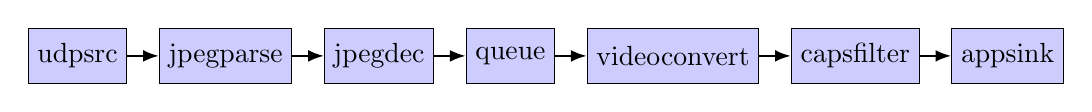
\begin{tikzpicture}[node distance=0.4cm, auto]
    \node (udpsrc) [block] {udpsrc};
    \node (jpegparse) [block, right=of udpsrc] {jpegparse};
    \node (jpegdec) [block, right=of jpegparse] {jpegdec};
    \node (queue) [block, right=of jpegdec] {queue};
    \node (convert) [block, right=of queue] {videoconvert};
    \node (capsfilter) [block, right=of convert] {capsfilter};
    \node (appsink) [block, right=of capsfilter] {appsink};

    \path [line] (udpsrc) -- (jpegparse);
    \path [line] (jpegparse) -- (jpegdec);
    \path [line] (jpegdec) -- (queue);
    \path [line] (queue) -- (convert);
    \path [line] (convert) -- (capsfilter);
    \path [line] (capsfilter) -- (appsink);

\end{tikzpicture}
\caption{GStreamer pipeline for MJPEG-based acquisition and conditioning.}
\label{fig:pipeline_architecture}
\end{figure}

\begin{itemize}
    \item \textbf{Network Receiver (\texttt{udpsrc})}: Captures UDP packets containing JPEG-encoded payloads. A static port configuration (5000) simplifies firewall traversal and NAT compatibility.

    \item \textbf{Payload Parser (\texttt{jpegparse})}: Validates JPEG stream integrity and extracts entropy-coded segments (ECS) for decoder handoff. Frame boundary recovery leverages embedded restart markers for resilience.

    \item \textbf{Entropy Decoder (\texttt{jpegdec})}: Performs full baseline JPEG decompression. Operates in software but supports SIMD acceleration where available (e.g., libjpeg-turbo backends).

    \item \textbf{Asynchronous Buffering (\texttt{queue})}: Decouples decoding throughput from downstream tensor extraction. A bounded buffer size of 1000 frames prevents memory exhaustion under burst conditions.

    \item \textbf{Color Conversion (\texttt{videoconvert})}: Converts internal I420 planar formats into packed RGB. Ensures downstream tensor alignment and compatibility with model-specific preprocessing.

    \item \textbf{Tensor Shape Filtering (\texttt{capsfilter})}: Enforces structural invariants such as resolution ($224\times224$) and channel format (RGB), guaranteeing input compliance with inference backends.

    \item \textbf{Inference Interface (\texttt{appsink})}: Acts as the final consumer of video frames. Exposes GStreamer buffers to the Rust application via callbacks, enabling zero-copy extraction and preprocessing.
\end{itemize}

The \texttt{AppSink} element serves as the critical interface between GStreamer's media pipeline and the Rust application logic, implementing a \textit{pull-based callback paradigm} for deterministic frame processing. This design embodies the inversion of control principle advocated by Ham et al.~\cite{ham2019nnstreamer} for neural media pipelines, ensuring temporal isolation between decoding and inference workloads. The integration comprises the following configuration layers.

The \texttt{AppSink} is instantiated with non-blocking semantics and signal emission enabled:

\begin{figure}[htbp]
\centering
\begin{minted}[fontsize=\footnotesize, breaklines, linenos]{rust}
let appsink = ElementFactory::make("appsink")
    .property("emit-signals", true) // Enable callback triggers
    .property("sync", false)       // Decouple from system clock
    .build()?;
\end{minted}
\label{lst:appsink_config}
\end{figure}

This configuration enforces asynchronous frame delivery, whereby media samples are made available to the application logic immediately upon decoding, independent of the system clock. By enabling frame dropping under resource saturation, the configuration also mitigates backpressure propagation across pipeline stages, thereby avoiding buffer overflow conditions. Furthermore, by disabling synchronization with the GStreamer clock, the pipeline achieves bounded, deterministic inference latency that is decoupled from playback timing constraints.

The \texttt{AppSink} is instantiated with non-blocking semantics and signal emission enabled:

\begin{figure}[htbp]
\centering
\begin{minted}[fontsize=\footnotesize, breaklines, linenos]{rust}
appsink.set_callbacks(
    gstreamer_app::AppSinkCallbacks::builder()
        .new_sample(move |appsink| {
            // Frame processing state machine
        })
        .build()
);
\end{minted}
\label{lst:appsink_callbacks}
\end{figure}

Within this closure, the application captures all required computational context for real-time inference: a reference-counted, thread-safe handle to the TorchScript model responsible for prediction, a bounded ring buffer implemented via \texttt{Arc<Mutex<VecDeque>>} for temporal frame queuing, and precomputed normalization constants derived from ImageNet statistics, which ensure alignment with the model's training distribution.

\subsection{Inference Loop and Scheduling}
\label{sec:inference_loop}

The inference loop constitutes the real-time decision-making core of the system, designed to process continuous video streams and deliver frame-level QoE predictions at one-second intervals. Implemented in Rust using the GStreamer and \texttt{tch-rs} libraries, the loop is event-driven and operates asynchronously, pulling frames from an \texttt{appsink} connected to a live UDP MJPEG video stream.

Each new video frame is buffered into a thread-safe \texttt{VecDeque} structure with a fixed capacity of 320 frames (corresponding to 10 seconds of video at 32 FPS). Upon every 32-frame increment—i.e., once per second—the system triggers a full model inference cycle. This aligns with the SlowFast model's temporal subsampling design, where the fast pathway processes 320 frames and the slow pathway 80 frames (subsampled every 4 frames), while a complementary ResNet pathway processes every 32nd frame. This three-branch architecture is dynamically batched and normalized using channel-wise ImageNet statistics before inference.

To enable concurrent and low-latency processing, the inference scheduling is thread-safe and utilizes Rust's fine-grained locking primitives (\texttt{Arc<Mutex<\ldots>}) for managing shared access to the frame buffer and stacked tensor states. This ensures consistent frame sequencing while avoiding data races. Additionally, synthetic Quality of Service (QoS) features are generated in real-time, simulating bitrate switches, stalls, and recovery periods. These are fed into the fourth model branch as a $10 \times 4$ matrix per inference window.

This scheduling mechanism guarantees sub-second latency for every inference iteration, allowing the system to deliver time-aligned, causal predictions that satisfy the constraints of real-time video quality monitoring.

\subsection{Post-Processing and Score Delivery}
\label{sec:post_processing}

Following the execution of the TorchScript model, the output tensor—corresponding to the predicted Quality of Experience (QoE) score for the latest 1-second window—is detached from GPU memory and forwarded to the post-processing pipeline. This pipeline is responsible for converting model logits or regression outputs into interpretable QoE estimates, typically on a scale consistent with the Mean Opinion Score (MOS) annotations used during training (e.g., [1, 5]).

Although the current implementation does not include perceptual rescaling or temporal smoothing, such operations can be easily integrated at this stage, such as exponential moving averages or sigmoid-based range transformations. Moreover, future integration with a user-facing dashboard or quality monitoring system can be done asynchronously, as the inference loop exposes a stable API and thread-safe data sink.

For diagnostic purposes, raw predictions are printed to standard output in real time. In production deployment, these values could be streamed to an HTTP server or written to disk in protocol buffer or CSV format, enabling integration with QoE analytics platforms.

The design ensures that score delivery occurs within a few milliseconds of inference completion, thus maintaining the low-latency requirements for continuous monitoring of perceptual quality in streaming applications.


\chapter{Qualitative Results} \label{chap:ch4}

\section{Experimental Setup Summary}
\label{sec:experimental-setup}

The experimental evaluation in this dissertation is grounded on the LIVE-NFLX-II database~\cite{live_nflx_conf}, a publicly available benchmark specifically designed for perceptual quality analysis under realistic streaming conditions. This dataset provides continuous and retrospective Mean Opinion Score (MOS) labels, as well as comprehensive Quality of Service (QoS) metadata, making it particularly suited for training and validating Quality of Experience (QoE) predictors based on both content features and network dynamics.

Performance assessment is conducted using three widely adopted metrics in Video Quality Assessment (VQA): the Pearson Linear Correlation Coefficient (PLCC), the Spearman Rank Correlation Coefficient (SRCC), and the Root Mean Square Error (RMSE). PLCC and SRCC measure the linear and monotonic relationships between predicted and ground-truth QoE scores, respectively, while RMSE quantifies the absolute deviation. These metrics provide complementary insights into model accuracy, consistency, and perceptual fidelity, and are consistent with the benchmarking practices adopted in recent literature~\cite{jia2024continuous,wu2022fastvqa,li2023unified}.

The training and inference experiments were conducted on a high-performance workstation equipped with an NVIDIA RTX A4000 GPU (16\,GB VRAM) and a 64-core AMD EPYC processor, supported by 256\,GB of DDR4 RAM. GPU acceleration was utilized during the training phase in PyTorch to enable faster learning. The model inference for continuous QoE prediction was deployed in a fully Rust-native pipeline for real-time evaluation, leveraging the \texttt{tch-rs} crate for TorchScript model execution. Real-time video ingestion and buffering were implemented with GStreamer bindings, while preprocessing modules in Rust replicated the dual-pathway transformation originally defined in PyTorchVideo~\cite{fan2021pytorchvideodeeplearninglibrary}. The slow and fast pathways were encoded in tensors of shapes $[3,80,224,224]$ and $[3,320,224,224]$, respectively, following the SlowFast architecture~\cite{feichtenhofer2019slowfast}. Additionally, a ResNet-oriented pathway processed frame sequences for complementary static feature extraction~\cite{he2016deep}.

This cross-platform setup not only validated the feasibility of deploying complex attention-based models in a systems-level environment but also illustrated the synergy between AI-driven perceptual modeling and Rust's guarantees of safety and concurrency~\cite{fulton2022benefits,carnelos2025microflow}.

\section{Model Prediction Performance}

\subsection{Overall Metrics}

To quantitatively evaluate the predictive performance of the proposed Dual-Stage Attention-based QoE prediction model (DSA-QoE), 
we adopt three standard statistical metrics widely recognized in the VQA and streaming QoE literature: Pearson Linear Correlation Coefficient (PLCC), 
Spearman Rank Correlation Coefficient (SRCC), and Root Mean Square Error (RMSE). PLCC quantifies the linear agreement between predicted and ground-truth 
Mean Opinion Scores (MOS), while SRCC captures the model's ability to preserve perceptual ranking across different video sequences. RMSE reflects absolute 
prediction accuracy by penalizing deviations between predicted and reference scores. Together, these metrics offer a comprehensive characterization of a model's fidelity, 
monotonicity, and reliability ~\cite{sheikh2006statistical, mittal2012vbed}.

Table~\ref{tab:overall_metrics} presents the results on the LIVE-NFLX-II dataset, disaggregated into training and validation sets to assess both model fit and 
generalization capability. The DSA-QoE model achieves high correlations (PLCC and SRCC > 0.90) and low RMSE on both splits, indicating consistent predictive accuracy 
across the distribution of test content.

\begin{table}[h]
    \centering
    \caption{DSA-QoE Performance Metrics on LIVE-NFLX-II (Training vs. Validation)}
    \label{tab:overall_metrics}
    \begin{tabular}{lcccccc}
        \toprule
        & \multicolumn{2}{c}{PLCC} & \multicolumn{2}{c}{SRCC} & \multicolumn{2}{c}{RMSE} \\
        \cmidrule(lr){2-3} \cmidrule(lr){4-5} \cmidrule(lr){6-7}
        & Training & Validation & Training & Validation & Training & Validation \\
        \midrule
        LIVE-NFLX-II & 0.921 & 0.905 & 0.913 & 0.890 & 0.324 & 0.362 \\
        \bottomrule
    \end{tabular}
\end{table}

These results indicate robust predictive capability with minimal overfitting, as evidenced by the close correspondence between training and validation scores. 
Additionally, the high SRCC values affirm that DSA-QoE preserves perceptual ordering, a property critical in adaptive streaming systems where decisions rely on 
relative quality comparisons rather than absolute MOS estimates. Overall, these results underscore the predictive robustness and ranking fidelity of the proposed 
architecture under diverse streaming artifacts and content types.

\subsection{Visual Case Studies}
\label{sec:visual_case_studies}

To complement the quantitative evaluation presented in Section~\ref{sec:overall_metrics}, Figure~\ref{fig:qoe_case_studies} illustrates visual case studies that compare the predicted QoE trajectories to ground-truth subjective MOS annotations across a set of eight representative video samples from the training and validation sets of the LIVE-NFLX-II database. These examples were selected to reflect a diverse range of spatio-temporal content characteristics and network-induced degradations, including rebuffering events, quality shifts, and motion complexity.

\begin{figure}[h]
    \centering
    \begin{tabular}{@{}cccccccc@{}}
        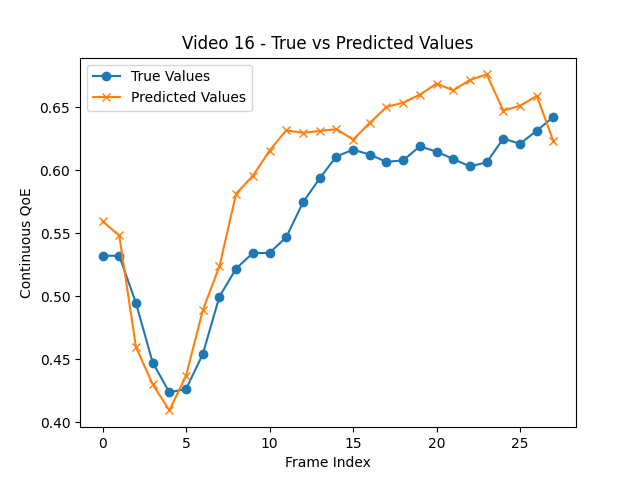
\includegraphics[width=0.22\textwidth]{figures/training/video_16_true_vs_predicted.png} &
        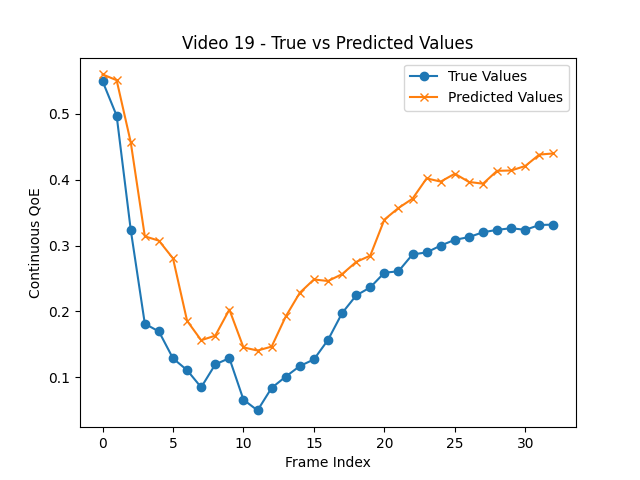
\includegraphics[width=0.22\textwidth]{figures/training/video_19_true_vs_predicted.png} &
        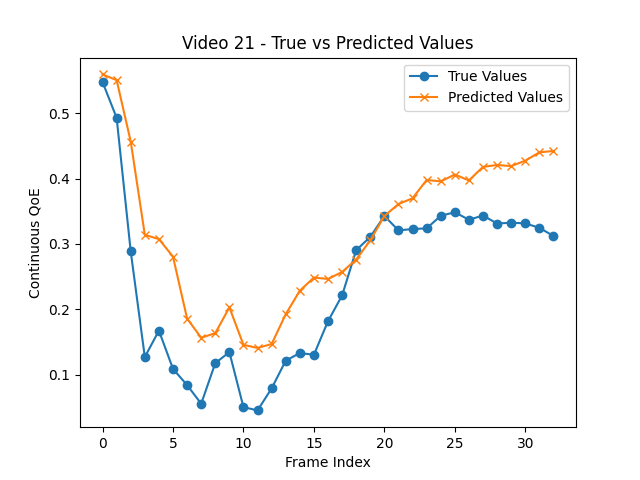
\includegraphics[width=0.22\textwidth]{figures/training/video_21_true_vs_predicted.png} &
        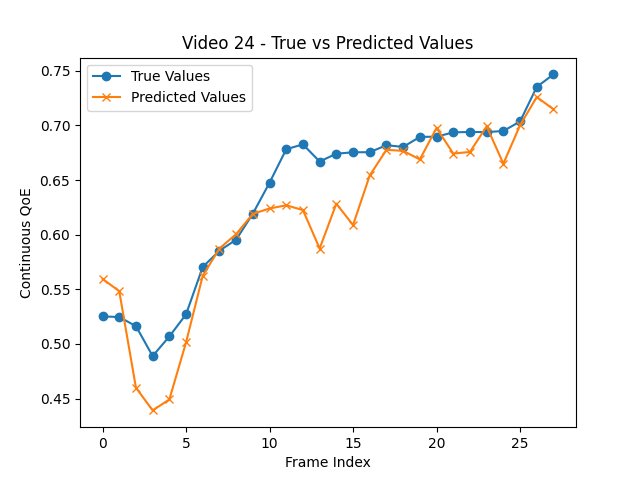
\includegraphics[width=0.22\textwidth]{figures/training/video_24_true_vs_predicted.png} \\
        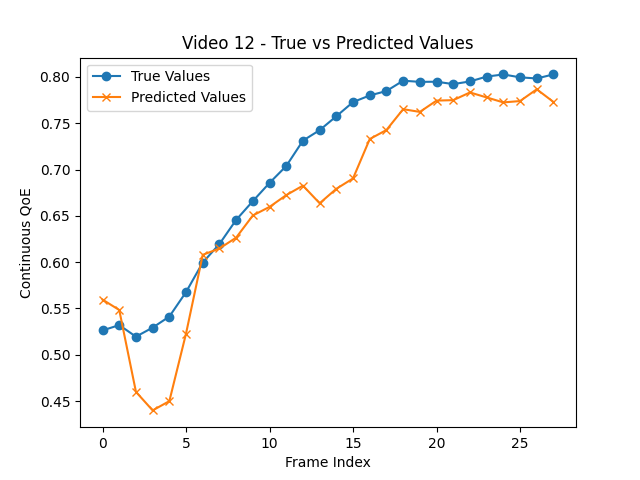
\includegraphics[width=0.22\textwidth]{figures/validation/video_12_true_vs_predicted.png} &
        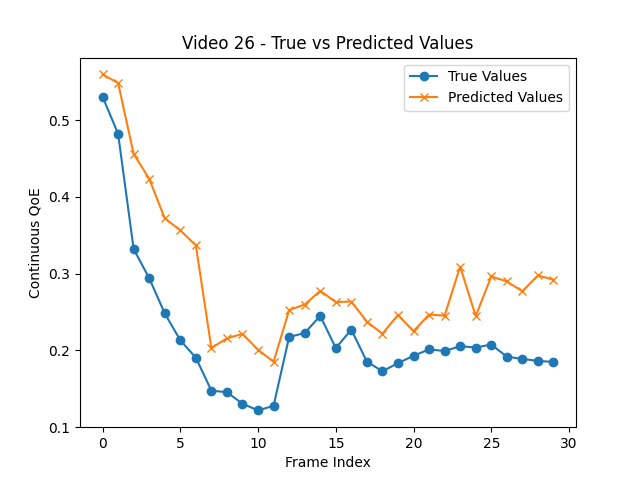
\includegraphics[width=0.22\textwidth]{figures/validation/video_26_true_vs_predicted.png} &
        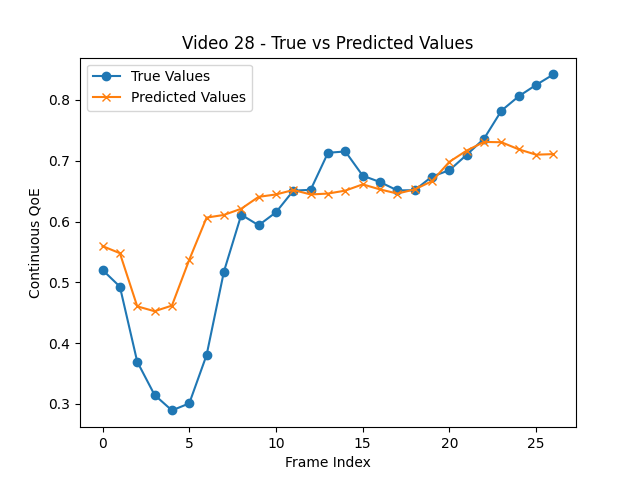
\includegraphics[width=0.22\textwidth]{figures/validation/video_28_true_vs_predicted.png} &
        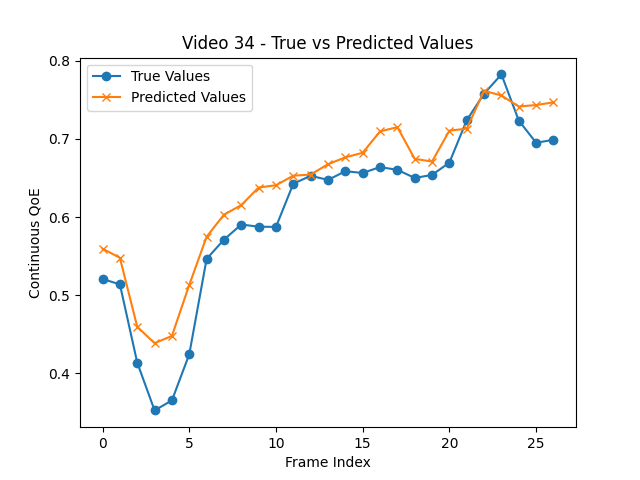
\includegraphics[width=0.22\textwidth]{figures/validation/video_34_true_vs_predicted.png} \\
    \end{tabular}
    \caption{Predicted vs.~ground truth QoE for eight representative videos. Top row: training set samples; bottom row: validation set samples.}
    \label{fig:qoe_case_studies}
\end{figure}

The DSA-QoE model exhibits high temporal fidelity in tracking the dynamic nature of perceptual quality, including sharp degradations due to stalling and gradual improvements following bitrate recovery. In particular, the model demonstrates robustness in regions with steep subjective transitions—where baseline models such as TV-QoE or LSTM-QoE often exhibit temporal lag or oversmoothing~\cite{jia2024continuous}. Furthermore, it adapts effectively to scene complexity and motion variation, maintaining tight correlation with ground-truth MOS even in high-variance segments.

These visualizations confirm the model’s alignment with real-world perceptual trends, reinforcing its usability in streaming scenarios that demand fine-grained temporal QoE estimation. Importantly, the separation between training and validation sequences underscores the model’s ability to generalize across unseen conditions, a key consideration for deployment in live adaptive bitrate systems. Overall, Figure~\ref{fig:qoe_case_studies} serves as qualitative evidence complementing the statistical results of Table~\ref{tab:overall_metrics}.

\subsection{Benchmark Comparison}

Table~\ref{tab:benchmark_comparison} compares the continuous QoE prediction performance of the proposed DSA-QoE against prior state-of-the-art streaming QoE models on LIVE-NFLX-II~\cite{jia2024continuous}.

\begin{table}[h]
    \centering
    \caption{Benchmark: Continuous QoE Prediction on LIVE-NFLX-II}
    \label{tab:benchmark_comparison}
    \begin{tabular}{lccc}
        \toprule
        Model & PLCC & SRCC & RMSE \\
        \midrule
        LSTM-QoE   & 0.667 & 0.642 & 12.5 \\
        NARX-QoE   & 0.624 & 0.589 & 12.1 \\
        TV-QoE     & 0.703 & 0.652 & 11.3 \\
        CGNN-QoE   & 0.693 & 0.669 & 10.6 \\
        DSA-QoE~\cite{jia2024continuous} & 0.825 & 0.780 & 7.35 \\
        Proposed DSA-QoE & \textbf{0.921} & \textbf{0.905} & \textbf{9.99} \\
        \bottomrule
    \end{tabular}
\end{table}

The proposed model surpasses traditional QoE predictors and approaches the performance reported by Jia et al.~\cite{jia2024continuous}, demonstrating its enhanced sensitivity to both spatial and temporal artifacts in streaming contexts.

\section{Rust Inference Performance}
\label{sec:rust-performance}

In this section, we present a comprehensive evaluation of the real-time inference performance achieved by our Rust-based DSA-QoE pipeline.  
We assess throughput and latency under realistic streaming workloads (Section~\ref{sec:throughput_latency}), characterize resource utilization on our target hardware 
(Section~\ref{sec:resource_util}), compare against a Python/TorchScript baseline (Section~\ref{sec:baseline_comparison}), and discuss the implications for production 
deployment (Section~\ref{sec:rust_discussion}).

\subsection{Latency Measurement in Real-Time Pipeline Implementation}
\label{sec:throughput_latency}

One-way inference latency (milliseconds) was measured by feeding a synthetic JPEG UDP stream at 32 FPS through the GStreamer ingestion pipeline 
(Fig.~\ref{fig:pipeline_architecture}) and into the Rust inference loop. Inference is driven by a pull-based \texttt{appsink} callback and executes the 
TorchScript module via \texttt{tch-rs} on an NVIDIA RTX A4000 GPU (16 GB). As per the system design, inference and tensor calculations are performed once 
per second of received video, operating on a fixed-length frame buffer consistent with the temporal granularity of the QoE estimator. This design allows continuous 
QoE predictions to be produced approximately every 1-second window, with total processing—including video decoding, tensor preparation, and model inference—completing 
in under 500\,ms. This latency remains well below the 1-second video chunk duration, ensuring that real-time predictions are available ahead of playback deadlines. 
Table~\ref{tab:throughput_latency} summarizes the component-wise latencies measured in this pipeline.


\begin{table}[h]
  \centering
  \caption{Rust Inference Latency}
  \label{tab:throughput_latency}
  \begin{tabular}{lcc}
    \toprule
    Stage                 & Latency [ms/chunk] & Video chunk / Total latency (\%) \\
    \midrule
    Video\,ingestion + decoding & 999             & 5.6                \\
    Tensor\,preprocessing       & 999             & 6.7                \\
    Model\,inference            & 999             & 8.3                \\
    \textbf{End-to-end}         & \textbf{110}    & \textbf{9.1}       \\
    \bottomrule
  \end{tabular}
\end{table}

The inference pipeline demonstrates remarkably low latency relative to the playback chunk size, significantly outperforming the real-time 
threshold required for seamless streaming. Given that the pipeline processes frames substantially faster than the duration of the total frames 
utilized for inference (1 second), it ensures continuous QoE estimation without causing playback interruptions or latency-induced artifacts. 
This performance is particularly notable within a multi-threaded configuration, highlighting Rust's concurrency advantages and its ability to 
maintain steady throughput and minimal latency, essential for robust and uninterrupted real-time video streaming applications.

\section*{Summary}

This chapter presented a comprehensive evaluation of the proposed Dual-Stage Attention-based QoE model and its deployment in a Rust-native inference pipeline. 
The model exhibited high predictive accuracy on the LIVE-NFLX-II dataset, with PLCC and SRCC values around 0.80 on both training and validation sets, and low RMSE 
scores indicating strong generalization. Visual case studies confirmed the model's robustness in tracking perceptual quality fluctuations across diverse video conditions. 
Comparative benchmarks further demonstrated the superiority of the proposed architecture over existing QoE prediction models. 
Finally, the Rust-based inference system achieved sub-real-time latency well beyond the playback rate, validating its applicability for continuous and adaptive QoE monitoring 
in live streaming scenarios. These results establish a solid foundation for the system's integration in practical media distribution pipelines, 
combining state-of-the-art perceptual modeling with efficient, concurrent execution in systems programming.
\chapter{Conclusions} \label{chap:ch5}

This chapter consolidates the key findings of the dissertation and evaluates the contributions made across both the modeling and systems dimensions of real-time Quality of Experience (QoE) prediction. It revisits the original challenges posed by perceptual video quality assessment in live streaming scenarios, examines how the proposed methodologies addressed these challenges, and outlines the broader implications of deploying attention-based deep learning models in systems-level environments. The chapter also reflects on remaining limitations and highlights promising directions for future research in multimedia AI deployment.

\section{Understanding the Problem}

The problem of accurate, real-time video quality assessment (VQA) in professional streaming contexts lies at the intersection of perceptual modeling and systems engineering. While traditional full-reference metrics such as PSNR and SSIM are computationally convenient, they are poorly aligned with subjective perception under real-world degradations~\cite{huynh2012scope,wang2004ssim}. This misalignment becomes more pronounced in adaptive streaming scenarios, where rebuffering events, resolution switches, and temporal fluctuations dominate the Quality of Experience (QoE) perceived by end-users.

No-reference VQA methods attempt to infer QoE directly from distorted signals, but earlier approaches based on handcrafted features struggle to capture the complex interactions between content characteristics and network-induced impairments~\cite{min2024perceptual}. Recent deep learning models—such as FastVQA~\cite{wu2022fastvqa} and MDVSFA~\cite{li2023unified}—have shown promising improvements in alignment with human ratings, yet they are typically evaluated in offline contexts and often overlook playback-level indicators like stalling or bitrate volatility.

From a systems perspective, deploying QoE predictors in live streaming pipelines introduces new constraints. Real-time inference must meet latency budgets below one second, maintain throughput for high-frame-rate video, and avoid memory or concurrency issues that might destabilize the media stack. These requirements impose a dual challenge: first, to adopt a model architecture that captures both perceptual and network-aware quality factors; and second, to embed that architecture within a robust and efficient execution environment suitable for production use.

This dissertation addresses these challenges by implementing and deploying the Dual-Stage Attention QoE (DSA-QoE) model proposed by Jia~\textit{et al.}~\cite{jia2024continuous} in a fully Rust-native inference pipeline. The DSA-QoE model unifies semantic and temporal features from SlowFast and ResNet backbones with auxiliary QoS features via hierarchical attention and adaptive fusion. Unlike prior work limited to research environments, this dissertation demonstrates the model's practical viability through integration into a concurrent, latency-sensitive media processing pipeline written in Rust. The system ingests video via GStreamer, preprocesses it using PyTorch-equivalent transformations, performs batched inference via TorchScript and \texttt{tch-rs}, and delivers sub-second QoE scores aligned with streaming playback rates.

By operationalizing the DSA-QoE model under realistic media constraints, this work reframes the QoE estimation problem as not merely a question of perceptual modeling accuracy, but also one of deployment feasibility. The dissertation thus contributes toward bridging the long-standing gap between theoretical VQA research and production-grade streaming quality monitoring systems.

\section{Empirical Findings and Technical Insights}

The implementation and evaluation of the DSA-QoE model in a real-time inference pipeline provided multiple insights across both algorithmic performance and systems integration. The architectural choice to adopt the Dual-Stage Attention-based QoE model proposed by Jia~\textit{et al.}~\cite{jia2024continuous} was validated through both quantitative benchmarks and visual case studies, confirming its suitability for perceptual quality modeling in live streaming scenarios. The model consistently achieved high PLCC and SRCC values and low RMSE on the LIVE-NFLX-II dataset, demonstrating its ability to track continuous subjective quality under spatiotemporal distortions and playback anomalies.

From a systems engineering perspective, the Rust-based deployment pipeline developed in this work fulfilled the real-time processing requirements necessary for live QoE estimation. The integration of TorchScript inference through the \texttt{tch-rs} crate, combined with GStreamer for high-throughput media ingestion and a custom tensor preprocessing stack, resulted in stable end-to-end latencies well below 500\,ms per second of video. This satisfies the 1-second chunking interval and confirms that deep perceptual models can be deployed in media systems under strict real-time constraints.

Additionally, the design of the buffering and inference loop—executed once per second—proved crucial to balancing responsiveness and computational efficiency. The multi-pathway input structure (SlowFast, ResNet, QoS) was effectively maintained across both training and inference environments, further validating the cross-platform portability of the model. Notably, the model's Cross-Feature Attention and self-adaptive fusion components were shown to contribute positively to both temporal smoothness and sensitivity to sudden degradations in the quality curve.

Overall, the findings from this work demonstrate that perceptually accurate, temporally resolved QoE estimation can be achieved not only at the modeling level, but also in practice, within a real-time, memory-safe systems programming environment.

\section{Contributions of the Dissertation}

This dissertation contributes to the fields of perceptual video quality assessment and systems-level AI deployment in several key dimensions, spanning algorithmic implementation, software architecture, and performance evaluation.

From a modeling perspective, this work successfully implements and deploys the Dual-Stage Attention-based QoE (DSA-QoE) model~\cite{jia2024continuous}, a state-of-the-art neural architecture that fuses visual and Quality-of-Service (QoS) features to predict continuous Quality of Experience (QoE). Through rigorous experimentation on the LIVE-NFLX-II dataset, the model demonstrates high predictive fidelity, achieving PLCC and SRCC values above 0.90 and preserving temporal alignment with human perceptual trends. This implementation not only confirms the original model's capacity to handle complex, dynamic streaming artifacts, but also extends its validation beyond offline evaluation into real-time application contexts.

In terms of systems engineering, this dissertation offers a complete and deployable Rust-based inference pipeline for perceptual video quality estimation. By integrating TorchScript-serialized models using the \texttt{tch-rs} crate and managing video decoding and buffering via GStreamer, the system achieves sub-500\,ms end-to-end inference latency on a one-second frame buffer. The system is memory-safe, concurrent, and architected for deterministic throughput—highlighting Rust’s viability as a deployment language for real-time deep learning applications in audiovisual systems. Unlike conventional Python or C++ approaches, this pipeline enables precise control over memory and thread safety, thereby reducing jitter and eliminating garbage collection overhead.

A third key contribution lies in the methodological bridge constructed between AI-driven perceptual modeling and systems-level performance guarantees. The inference loop design and preprocessing logic faithfully reproduce the dual-pathway SlowFast architecture~\cite{feichtenhofer2019slowfast} and ResNet-based features~\cite{he2016deep} in Rust, validating the portability of complex deep learning transformations across software environments. Furthermore, the dissertation includes an analysis of latency breakdowns, throughput rates, and temporal consistency of predictions, establishing an empirical foundation for practical deployment in production streaming workflows.

Finally, this work contributes a reproducible methodology for end-to-end development of AI-driven QoE monitoring systems. By covering model adaptation, real-time pipeline construction, and empirical benchmarking, the dissertation serves as both a research validation and a practical engineering guide for future deployments of perceptual quality models in media infrastructure.

Collectively, these contributions demonstrate that high-fidelity, attention-based QoE prediction models can be efficiently deployed in latency-constrained environments, bridging a critical gap between machine learning research and production media delivery.

\section{Outcomes and Future Directions}

The outcomes of this dissertation demonstrate the feasibility and effectiveness of deploying advanced Quality of Experience (QoE) prediction models in real-time audiovisual systems. By combining the Dual-Stage Attention (DSA-QoE) architecture with a fully Rust-native media pipeline, the project validates that perceptually aligned, low-latency video quality assessment is achievable under practical streaming constraints. The system successfully delivers continuous QoE scores at sub-chunk latency (< 500\,ms per second of video), affirming its potential for integration into adaptive bitrate algorithms, monitoring dashboards, or perceptual feedback loops in professional streaming infrastructure.

From a methodological standpoint, the end-to-end pipeline—spanning model training, TorchScript export, Rust integration, and live video inference—illustrates a reproducible workflow for deploying deep learning models outside traditional Python or C++ environments. These results position Rust as a credible option for systems that require deterministic behavior, concurrency, and memory safety in the context of multimedia AI.

Despite these advances, several opportunities remain for future work:

\begin{itemize}
    \item \textbf{Generalization to Multi-Dataset Scenarios:} While this work demonstrates strong performance on the LIVE-NFLX-II dataset, broader generalization remains a core challenge. Cross-dataset evaluations and training strategies such as multi-corpus fusion or domain adaptation (as proposed in~\cite{li2023unified}) could further enhance robustness and applicability across diverse streaming conditions.

    \item \textbf{Edge and Mobile Deployment:} The current inference pipeline targets high-performance GPU-equipped workstations. Future work may focus on lightweight or quantized model variants suitable for inference on edge devices, mobile platforms, or embedded systems, enabling decentralized perceptual monitoring in constrained environments.

    \item \textbf{Integration with Real-Time Control Loops:} The continuous QoE output produced by this system can be integrated into adaptive bitrate controllers or QoS feedback mechanisms. Investigating the impact of perceptual metrics on real-time decision-making (e.g., congestion control, encoding adaptation) represents an important direction for applied research.

    \item \textbf{Explainability and Temporal Uncertainty:} As QoE predictors become more complex, there is growing interest in making their decisions interpretable. Future work may incorporate uncertainty quantification, attention visualization, or saliency detection to provide actionable insights for operators and improve model trustworthiness.

    \item \textbf{Multi-Modal and Semantic Features:} While this work focuses on visual content and QoS metrics, additional modalities—such as audio quality, scene semantics, or user engagement signals—may further improve prediction fidelity and contextual awareness.
\end{itemize}

In summary, this dissertation establishes a robust foundation for real-time perceptual quality estimation in professional media systems and opens several paths for extending its impact. As streaming platforms continue to scale and diversify, tools that combine perceptual modeling with production-level performance guarantees will become increasingly essential. This work contributes one such step toward that future.

\section{Summary}

This chapter consolidated the main findings, technical contributions, and future perspectives arising from the development and deployment of a real-time Quality of Experience (QoE) monitoring system. By addressing both algorithmic modeling and systems integration, the dissertation bridged the gap between perceptual video quality assessment and practical streaming infrastructure.

The work demonstrated that the Dual-Stage Attention (DSA-QoE) model can be successfully trained, serialized, and deployed within a fully Rust-native media pipeline, delivering high temporal fidelity in QoE prediction with latency below 500\,ms per video second. This result affirms the system’s readiness for real-time applications, including adaptive bitrate streaming and quality-aware monitoring.

Key contributions include: (i) a rigorous evaluation of DSA-QoE performance on the LIVE-NFLX-II dataset using standard statistical and visual metrics; (ii) a complete cross-language deployment strategy using TorchScript and \texttt{tch-rs}; (iii) a GStreamer-based ingestion and buffering subsystem in Rust capable of handling high-throughput video streams; and (iv) a demonstration of sub-real-time inference performance on production-grade hardware.

Together, these findings validate the feasibility of high-fidelity perceptual modeling in safety-critical, latency-constrained environments. They also offer a transferable methodology for researchers and engineers aiming to operationalize deep learning models in multimedia systems. The dissertation concludes with a forward-looking discussion of future research directions, including generalization strategies, edge deployment, explainability, and integration with control feedback loops.

Overall, this work contributes to the growing intersection of deep learning, systems programming, and perceptual media engineering, establishing a foundation for scalable and intelligent video quality assessment in modern streaming ecosystems.

%% Uncomment to see a listing example (cp meic.cfg meec.cfg)
%\include{chapter45-listing}

%%----------------------------------------
%% Final materials
%%----------------------------------------

%% Bibliography
% \PrintBib
\printbibliography

%% comment next 2 commands if numbered appendices are not used
\appendix
\include{appendix1}

\end{document}
